%DIF 1c1
%DIF LATEXDIFF DIFFERENCE FILE
%DIF DEL constructing_lin_eqns_2013-08-13.tex         Mon Aug 19 11:21:56 2013
%DIF ADD constructing_lin_eqns_2013-08-13_after.tex   Mon Aug 19 11:23:25 2013
%DIF < % Mon 19 Aug 2013 10:08:29 EDT
%DIF -------
% Mon 19 Aug 2013 10:08:29 EDT  with corrections %DIF > 
%DIF -------
\documentclass[twocolumn,10pt]{article}
\title{Constructing linear functions}

\setlength{\columnsep}{20pt} 
\usepackage{amsmath,hyperref,cancel,graphicx}
 \def\shrinkfactor{0.55}
 \usepackage[margin=1.5cm]{geometry}
\usepackage[usenames,dvipsnames]{color}
 
 \newcommand{\blue}[1]{{\color{Blue}#1}} 
 \newcommand{\purple}[1]{{\color{Purple}#1}} 
 \newcommand{\red}[1]{{\color{Red}#1}} 
 \newcommand{\green}[1]{{\color{Green}#1}} 
 \newcommand{\gray}[1]{{\color{Gray}#1}} 
  \newcommand{\pink}[1]{{\color{Magenta}#1}}   
%DIF PREAMBLE EXTENSION ADDED BY LATEXDIFF
%DIF UNDERLINE PREAMBLE %DIF PREAMBLE
\RequirePackage[normalem]{ulem} %DIF PREAMBLE
\RequirePackage{color}\definecolor{RED}{rgb}{1,0,0}\definecolor{BLUE}{rgb}{0,0,1} %DIF PREAMBLE
\providecommand{\DIFadd}[1]{{\protect\color{blue}\uwave{#1}}} %DIF PREAMBLE
\providecommand{\DIFdel}[1]{{\protect\color{red}\sout{#1}}}                      %DIF PREAMBLE
%DIF SAFE PREAMBLE %DIF PREAMBLE
\providecommand{\DIFaddbegin}{} %DIF PREAMBLE
\providecommand{\DIFaddend}{} %DIF PREAMBLE
\providecommand{\DIFdelbegin}{} %DIF PREAMBLE
\providecommand{\DIFdelend}{} %DIF PREAMBLE
%DIF FLOATSAFE PREAMBLE %DIF PREAMBLE
\providecommand{\DIFaddFL}[1]{\DIFadd{#1}} %DIF PREAMBLE
\providecommand{\DIFdelFL}[1]{\DIFdel{#1}} %DIF PREAMBLE
\providecommand{\DIFaddbeginFL}{} %DIF PREAMBLE
\providecommand{\DIFaddendFL}{} %DIF PREAMBLE
\providecommand{\DIFdelbeginFL}{} %DIF PREAMBLE
\providecommand{\DIFdelendFL}{} %DIF PREAMBLE
%DIF END PREAMBLE EXTENSION ADDED BY LATEXDIFF

\begin{document}
\maketitle



\section{\href{https://www.khanacademy.org/devadmin/content/items/x0901bc4c}{x0901bc4c}}

\noindent
A cyclist is riding downhill on a smooth road which starts at the top of a \DIFdelbegin \DIFdel{hill }\DIFdelend \DIFaddbegin \DIFadd{mountain }\DIFaddend and descends towards the ocean.
His height $h$ above the ocean level is a function of the distance $d$ from the top of the \DIFdelbegin \DIFdel{hill}\DIFdelend \DIFaddbegin \DIFadd{mountain}\DIFaddend .
The top of the \DIFdelbegin \DIFdel{hill }\DIFdelend \DIFaddbegin \DIFadd{mountain }\DIFaddend has a height of $h=1200\text{ m}$. For each $1000\text{ m}$ of distance traveled, 
his height $h$ decreases by $200\text{ m}$.

**Find the equation \DIFdelbegin \DIFdel{which }\DIFdelend \DIFaddbegin \DIFadd{that }\DIFaddend describes $h$ as a function of $d$.**

\paragraph{Ans}The equation \DIFdelbegin \DIFdel{which }\DIFdelend \DIFaddbegin \DIFadd{that }\DIFaddend describes the height $h$ as a function of the distance $d$ is   
[[? expression 1]] h = 1200 - 0.2d

\paragraph{Hint 1}We're given the description of a real-world situation and asked to find the mathematical equation \DIFdelbegin \DIFdel{which }\DIFdelend \DIFaddbegin \DIFadd{that }\DIFaddend describes it. We want to find the equation \DIFdelbegin \DIFdel{which }\DIFdelend \DIFaddbegin \DIFadd{that }\DIFaddend describes the height of the cyclist $\blue{h}$ as a function of the distance $d$ traveled from the top of the \DIFdelbegin \DIFdel{hill}\DIFdelend \DIFaddbegin \DIFadd{mountain}\DIFaddend .

\paragraph{Hint 2}The initial height of the cyclist when he starts at the top of the \DIFdelbegin \DIFdel{hill }\DIFdelend \DIFaddbegin \DIFadd{mountain }\DIFaddend is $\green{1200}\text{ m}$. This height corresponds to a distance of $\red{d}=0\text{ m}$ from the starting point.

\paragraph{Hint 3}Now let's find the rate of change of the height of the cyclist as he travels down the \DIFdelbegin \DIFdel{hill}\DIFdelend \DIFaddbegin \DIFadd{mountain}\DIFaddend . We are told that for each $\red{1000}\text{ m}$ of distance traveled, 
his height $\blue{h}$ decreases by $\blue{200}\text{ m}$. We calculate the rate of change of the height function by dividing the  \DIFdelbegin \DIFdel{the }\DIFdelend change in the height by the change in the distance:

$\quad \purple{m} = \dfrac{ \textrm{change in } \blue{h} }{ \textrm{change in } \red{d} } = \dfrac{ \blue{-200} }{ \red{1000} } = \purple{-0.2}$.

For each meter of distance traveled, the height of the cyclist decreases by $\purple{0.2}$ meters.

\paragraph{Hint 4}The equation \DIFdelbegin \DIFdel{which }\DIFdelend \DIFaddbegin \DIFadd{that }\DIFaddend describes the height $\blue{h}$ of the cyclist as a function of the distance $\red{d}$ is the following:

\begin{align*}
\quad \blue{h} &= \green{1200} -  \purple{0.2}\red{d}.
\end{align*}

Note that the height $\blue{h}$ is described by a *linear equation* $\blue{h}=\green{b}+ \purple{m}\cdot\red{d}$, where $\green{b}=\green{1200}$ represents the initial height and $\purple{m}=\purple{-0.2}$ represents the rate of change of the height.

\paragraph{Hint 5}The equation \DIFdelbegin \DIFdel{which }\DIFdelend \DIFaddbegin \DIFadd{that }\DIFaddend describes $h$ as a function of $d$ is $h= 1200-0.2d$.



\medskip
\noindent
\textbf{Tags:} {\footnotesize CC.8.F.B.4, SB.8.1.F.1.CR, Constructing linear functions.1}\\
\textbf{Version:} \DIFdelbegin \DIFdel{9cb40256.. 2013-08-12
}\DIFdelend \DIFaddbegin \DIFadd{145f0668.. 2013-08-19
}\DIFaddend \smallskip\hrule





\section{\href{https://www.khanacademy.org/devadmin/content/items/x0b401d79}{x0b401d79}}

\noindent
David is visiting San Francisco. He wants to rent a bicycle for a couple of hours to be able to better explore the city. The price of the rental includes a base charge of $\$10$ and an additional charge of $\$4$ per hour.

**Write the function \DIFdelbegin \DIFdel{which }\DIFdelend \DIFaddbegin \DIFadd{that }\DIFaddend represents the price $P\:$  for $h$ hours of bike rental.**    

\paragraph{Ans}The price of the rental $P\:$ as a function of the number of hours $h$ is   
[[? expression 1]]  P = 10+4*h

\paragraph{Hint 1}Let's use the information provided to figure out the function \DIFdelbegin \DIFdel{which }\DIFdelend \DIFaddbegin \DIFadd{that }\DIFaddend describes the price $\blue{P}\:$ of the bike rental.

The bike rental includes a fixed charge of $\$\green{10}$. This is the base amount David has to pay to rent out the bicycle.

To find the total price, we have to add the \DIFdelbegin \DIFdel{hourly charge which is }\DIFdelend \DIFaddbegin \DIFadd{base price to the hourly charge of }\DIFaddend $\$\purple{4}$ per hour. If David rents the bike for $\red{h}$ hours, the hourly charge will be $\purple{4}\red{h}$ dollars.

\paragraph{Hint 2}The price of the bike rental is described by the following equation:

$\quad \blue{P} = \green{10} + \purple{4}\red{h}$.

Note the price function corresponds to a linear equation $\blue{P}=\green{b}+\purple{m}\red{h}$.
The number $\green{b}$ corresponds to the fixed price of the bike rental, which is $\$\green{10}$.
The number $\purple{m}=\purple{4}$ corresponds to the hourly rate.

\paragraph{Hint 3}The price of the rental $P\:$ for $h$ hours is $P= 4h + 10$ dollars.



\medskip
\noindent
\textbf{Tags:} {\footnotesize CC.8.F.B.4, SB.8.1.F.1.CR, Constructing linear functions.1}\\
\textbf{Version:} \DIFdelbegin \DIFdel{1326b562.. 2013-08-08
}\DIFdelend \DIFaddbegin \DIFadd{70b4748f.. 2013-08-19
}\DIFaddend \smallskip\hrule





\section{\href{https://www.khanacademy.org/devadmin/content/items/x13c34d60}{x13c34d60}}

\noindent
Arlo is setting up a rooftop garden with vegetables. He has a budget of $\$80$ for this project. He drives to a local farm to buy the plants. The farmer offers to sell him pepper plants for $\$2$ each and tomato plants for $\$3$ each.

Assume that Arlo wants to spend the *entire* budget at this farm. **Write an equation \DIFdelbegin \DIFdel{which }\DIFdelend \DIFaddbegin \DIFadd{that }\DIFaddend describes the  number of pepper plants $p$ as a function of the  number of tomato plants $t$ that Arlo can buy.**

\paragraph{Ans}The \DIFaddbegin \DIFadd{equation that describes the }\DIFaddend number of pepper plants $p$ \DIFdelbegin \DIFdel{and }\DIFdelend \DIFaddbegin \DIFadd{as a function of }\DIFaddend the number of tomato plants $t$ \DIFdelbegin \DIFdel{are related by the equation
 }\DIFdelend \DIFaddbegin \DIFadd{is
 }\DIFaddend [[? expression 1]] p = 40 - (3/2)*t

\paragraph{Hint 1}We're trying to find \DIFdelbegin \DIFdel{an equation which }\DIFdelend \DIFaddbegin \DIFadd{the equation that }\DIFaddend relates the number of pepper plants $\green{p}$ and the number of tomato plants $\red{t}$ that Arlo can buy for *exactly* $\$80$.

\paragraph{Hint 2}The price for each pepper plant is $\$2$, so the cost of $\green{p}$ pepper plants is $2\green{p}$ dollars.
The price of $\red{t}$ tomato plants is $3\red{t}$ dollars.
The total budget for purchasing the plants is $\$80$.

Since we know Arlo wants to spend exactly $\$80$, the equation \DIFdelbegin \DIFdel{which }\DIFdelend \DIFaddbegin \DIFadd{that }\DIFaddend describes the relationship between the number of pepper and tomato plants he can buy is

$\quad 80  = 2\green{p} + 3\red{t}$.

The individual numbers $\green{p}$ and $\red{t}$ can vary, but we know these numbers are *related* because the combined cost of the purchase needs to equal $\$80$.

\paragraph{Hint 3}We can also think of the number of pepper plants as a function of the number of tomato plants. If Arlo chooses to buy some number of tomato plants $\red{t}$, then the number of pepper plants $\green{p}$ will *depend* on the number $\red{t}$.

To find $\green{p}$ as a function of $\red{t}$ let's start with the original equation and rewrite it so that $\green{p}$ appears isolated on one side of the equation:

\begin{align*}
 \quad 2p + 3t   &= 80   \\[1mm]
2p + 3t \ \  \blue{-3t}     &= 80  \blue{-3t}   \\
2p     &= 80  - 3t   \\[2mm]
\blue{\dfrac{1}{2}}\left( 2p \right)     &= \blue{\dfrac{1}{2}}\left( 80  - 3t  \right) \\[1mm]
\green{p}     &= 40  - \frac{3}{2}\red{t}.
\end{align*}

Note how, in the above equations, we perform the same operation to the left-hand side and to the right-hand side of the equation. 

The equation $\green{p} = 40  - \frac{3}{2}\red{t}$ describes how the number of pepper plants depends on the number of tomato plants. If Arlo wants to buy $\red{t}=\red{10}$ tomato plants, he will be able to buy $\green{p} = 40  - \frac{3}{2}(\red{10}) = \green{25}$ pepper plants.

\paragraph{Hint 4}**The equations \DIFdelbegin \DIFdel{which describes $\green{p}$ }\DIFdelend \DIFaddbegin \DIFadd{that describes $p$ }\DIFaddend as a function of \DIFdelbegin \DIFdel{$\red{t}$ is $\green{p} = 40 -\frac{3}{2}\red{t}$}\DIFdelend \DIFaddbegin \DIFadd{$t$ is $p = 40 -\frac{3}{2}t$}\DIFaddend .**

\paragraph{Hint 5}Note that we could also start from the relation $2\green{p} + 3\red{t} = 80$ and isolate $\red{t}$ to obtain the equation $\red{t} = \frac{80}{3} - \frac{2}{3}\green{p}$. This equation describes $\red{t}$ as a function of $\green{p}$. In other words, we choose the number of pepper plants first, and then the number of tomato plants depends on that choice**.**



\medskip
\noindent
\textbf{Tags:} {\footnotesize CC.8.F.B.4, SB.8.1.F.1.CR, Constructing linear functions.1}\\
\textbf{Version:} \DIFdelbegin \DIFdel{aaa78399.. 2013-08-12
}\DIFdelend \DIFaddbegin \DIFadd{688e2a6c.. 2013-08-19
}\DIFaddend \smallskip\hrule





\section{\href{https://www.khanacademy.org/devadmin/content/items/x288363ab}{x288363ab}}

\noindent
Jane runs a company which manufactures bicycles. The operating costs of Jane's company are of two types. Each month, the company must cover the fixed costs of $\$3000$ for rent and utilities. The production costs are $\$100$ per bicycle.

**What is the equation \DIFdelbegin \DIFdel{which describes the }\DIFdelend \DIFaddbegin \DIFadd{that describes the total }\DIFaddend costs $C$ as a function of the number of bicycles produced $x$?**

\paragraph{Ans}The equation that describes $C$ as a function of $x$ is  
 [[? expression 1]] C=3000 + 100x

\paragraph{Hint 1}We're trying to find the equation \DIFdelbegin \DIFdel{which }\DIFdelend \DIFaddbegin \DIFadd{that }\DIFaddend corresponds to the operating costs $\blue{C}$ of Jane's company as a function of the number of bicycles produced $\red{x}$.
We know the fixed costs are $\$\green{3000}$ per month. Additionally, there is a production cost of $\$\purple{100}$ per bicycle.

\paragraph{Hint 2}The *fixed costs* of a company \DIFdelbegin \DIFdel{is the part of the }\DIFdelend \DIFaddbegin \DIFadd{are the }\DIFaddend costs that are present even when Jane's company does not produce any \DIFdelbegin \DIFdel{items }\DIFdelend \DIFaddbegin \DIFadd{bicycles }\DIFaddend $\red{x}=0$. We know that each month Jane has to pay $\green{3000}$ dollars for rent and utilities and that this number does not depend on the number of bicycles produced.

\paragraph{Hint 3}Now let's look at the variable costs. The *variable* costs of a company depend on the number of bicycles produced.

If Jane produces $\red{x}$ bicycles this month, her variable costs will be $\purple{100}\red{x}$ dollars, since each bicycle costs $\$\purple{100}$ to produce. 

\paragraph{Hint 4}The total of the costs of Jane's company is the sum of the fixed costs and the variable costs:

$\quad \blue{C}= \purple{100}\red{x} + \green{3000}$ dollars.

\paragraph{Hint 5}Note that the total costs of the company are described by a linear equation of the form $\blue{C}=\purple{m}\red{x}+\green{b}$, where the number $\purple{m}$ corresponds to the *unit cost of production*, and $\green{b}$ is the *initial value* of the \DIFaddbegin \DIFadd{costs }\DIFaddend function.

\paragraph{Hint 6}The equation that describes $C$ as a function of $x$  is $C = 100x + 3000$.



\medskip
\noindent
\textbf{Tags:} {\footnotesize CC.8.F.B.4, SB.8.1.F.1.CR, Constructing linear functions.1}\\
\textbf{Version:} \DIFdelbegin \DIFdel{d4fa81fe.. 2013-08-12
}\DIFdelend \DIFaddbegin \DIFadd{f50ded60.. 2013-08-19
}\DIFaddend \smallskip\hrule





\section{\href{https://www.khanacademy.org/devadmin/content/items/x464f53e1}{x464f53e1}}

\noindent
Jessica works in sales. Her monthly salary is calculated as a base amount of $\$2000$ plus a commission of $\$100$ for each sale she makes. Assume $n$ represents the number of sales Jessica makes, and $S$ represents her monthly salary.

**Find the equation \DIFdelbegin \DIFdel{which }\DIFdelend \DIFaddbegin \DIFadd{that }\DIFaddend represents Jessica's monthly salary $S$ as a function of the number of sales $n$.**

\paragraph{Ans}The equation \DIFdelbegin \DIFdel{which }\DIFdelend \DIFaddbegin \DIFadd{that }\DIFaddend describes $S$ as a function of $n$ is   
[[? expression 1]] S= 2000+100*n

\paragraph{Hint 1}We are told Jessica's salary $\blue{S}$ increases by $\$\purple{100}$ for each sale she makes. Also, we know that she receives a base amount of $\$\green{2000}$.  Let's see how we can use the information provided to figure out the function \DIFdelbegin \DIFdel{which }\DIFdelend \DIFaddbegin \DIFadd{that }\DIFaddend describes Jessica's monthly salary.

\paragraph{Hint 2}The initial value of the salary function is $\$\green{2000}$. This is the base amount Jessica earns even when she makes $\red{n}=0$ sales.

The rate of change of the salary function is $\$\purple{100}$ per sale because this is how much she makes per sale. If $\red{n}$ increases by one, her salary $\blue{S}$ will increase by $\$\purple{100}$. 

We can combine these two facts to find Jessica's monthly salary $\blue{S}$ as a function of the number of sales $\red{n}$:

 \begin{align*}
\quad \blue{S} &= \purple{100}\red{n}  + \green{2000}.
\end{align*}

\paragraph{Hint 3}Note that the salary $\blue{S}$ is described by a *linear equation* $\blue{S}=\purple{m}\cdot\red{n}  + \green{b}$, where $\green{b}=\green{2000}$ represents the initial value of the function and $\purple{m}=\purple{100}$ represents the rate of change of the function.

\paragraph{Hint 4}The equation \DIFdelbegin \DIFdel{which }\DIFdelend \DIFaddbegin \DIFadd{that }\DIFaddend describes $S$ as a function of $n$ is $S= 2000+100n$.



\medskip
\noindent
\textbf{Tags:} {\footnotesize CC.8.F.B.4, SB.8.1.F.1.CR, Constructing linear functions.1}\\
\textbf{Version:} \DIFdelbegin \DIFdel{d700ce83.. 2013-08-11
}\DIFdelend \DIFaddbegin \DIFadd{2595c11c.. 2013-08-19
}\DIFaddend \smallskip\hrule





\section{\href{https://www.khanacademy.org/devadmin/content/items/x4fde7439}{x4fde7439}}

\noindent
Monica manages a content company \DIFdelbegin \DIFdel{which }\DIFdelend \DIFaddbegin \DIFadd{that }\DIFaddend specializes in producing news articles \DIFdelbegin \DIFdel{that cover }\DIFdelend \DIFaddbegin \DIFadd{on }\DIFaddend scientific topics.
The company's staff writers produce $100$ articles each week.
In addition, Monica can hire contractors who produce $5$ articles each week.

**Write the equation \DIFdelbegin \DIFdel{which }\DIFdelend \DIFaddbegin \DIFadd{that }\DIFaddend describes the total number of articles produced by the company $N$,
as a function of the number of contractors hired $n$.**

\paragraph{Ans}The equation \DIFdelbegin \DIFdel{which }\DIFdelend \DIFaddbegin \DIFadd{that }\DIFaddend describes the number of articles  produced $N$ as a function of the number of contractors $n$ is   
[[? expression 1]] N = 100 + 5n

\paragraph{Hint 1}Let's use the information provided to figure out how many articles the content company \DIFdelbegin \DIFdel{will produce }\DIFdelend \DIFaddbegin \DIFadd{produces }\DIFaddend in total.

\paragraph{Hint 2}If Monica hires zero contractors, $\red{n}=0$, then only the staff writers will write articles so the total amount of articles will be $\green{100}$. 

Each of the contractors Monica hires will produce $\purple{5}$ articles per week, so if Monica hires $\red{n}$ contractor writers\DIFaddbegin \DIFadd{, }\DIFaddend they will produce  $\purple{5}\red{n}$ additional articles.

\paragraph{Hint 3}To find the total number of articles produced by Monica's company, we must combine the articles produced by the staff writers and the articles produced by the contractors.

The number of articles $\blue{N}$ produced when  $\red{n}$ contractors are hired will be 

\begin{align*}
\quad \blue{N} &= \green{100} +  \purple{5}\red{n}.
\end{align*}

Note that the number of articles $\blue{N}$ is described by a *linear equation* $\blue{N}=\green{b}+ \purple{m}\cdot\red{n}$, where $\green{b}=\green{100}$ represents the initial value of the function, and $\purple{m}=\purple{5}$ represents the increase in the number of articles produced by hiring more contractors.

\paragraph{Hint 4}The equation \DIFdelbegin \DIFdel{which }\DIFdelend \DIFaddbegin \DIFadd{that }\DIFaddend describes $N$ as a function of $n$ is $N= 100+5n$.



\medskip
\noindent
\textbf{Tags:} {\footnotesize CC.8.F.B.4, SB.8.1.F.1.CR, Constructing linear functions.1}\\
\textbf{Version:} \DIFdelbegin \DIFdel{76b74a92.. 2013-08-13
}\DIFdelend \DIFaddbegin \DIFadd{3d21142f.. 2013-08-19
}\DIFaddend \smallskip\hrule





\section{\href{https://www.khanacademy.org/devadmin/content/items/x53c38ae0}{x53c38ae0}}

\noindent
Frida receives $\$10$ in pocket money from her parents each week.
She uses some of this money to buy ice cream (there is a really good ice cream shop near her house),
and puts the remaining money in her piggy bank. 
If she saves enough, one day she will be able to buy the whole ice cream shop!

Let $n$ represent the number of ice cream cones Frida buys this week,
and let $s$ represent the amount of saved money Frida has left to put in the piggy bank this week.
Each ice cream cone costs $\$1.5$.  
**What is the equation \DIFdelbegin \DIFdel{which }\DIFdelend \DIFaddbegin \DIFadd{that }\DIFaddend describes $s$ as a function of $n$?**

\paragraph{Ans}The equation \DIFdelbegin \DIFdel{which }\DIFdelend \DIFaddbegin \DIFadd{that }\DIFaddend describes the savings $s$ \DIFdelbegin \DIFdel{which remain }\DIFdelend \DIFaddbegin \DIFadd{remaining }\DIFaddend after Frida buys $n$ ice cream cones is 
[[? expression 1]] s = 10 - 1.5n

\paragraph{Hint 1}We are told Frida's allowance is $\$\green{10}$ and that each ice cream cone costs $\$\purple{1.5}$. 
We want to find the equation \DIFdelbegin \DIFdel{which }\DIFdelend \DIFaddbegin \DIFadd{that }\DIFaddend describes Frida's saved money $s$ as a function of the number of ice cream cones she buys. 

\paragraph{Hint 2}The maximum savings Frida can add to her piggy bank is $\$\green{10}$. This corresponds to the case when she buys $\red{n}=0$ ice cream cones.

\paragraph{Hint 3}To find the savings $\blue{s}$ for a given week, we must subtract the money spent on ice cream from the initial value of $\$\green{10}$. We obtain the following equation:

 \begin{align*}
\quad \blue{s} &= \green{10} -  \purple{1.5}\red{n}.
\end{align*}

\paragraph{Hint 4}The equation \DIFdelbegin \DIFdel{which }\DIFdelend \DIFaddbegin \DIFadd{that }\DIFaddend describes $s$ as a function of $n$ is $s= 10-1.5n$.



\medskip
\noindent
\textbf{Tags:} {\footnotesize CC.8.F.B.4, SB.8.1.F.1.CR, Constructing linear functions.1}\\
\textbf{Version:} \DIFdelbegin \DIFdel{7e9a21b4.. 2013-08-13
}\DIFdelend \DIFaddbegin \DIFadd{0b8908be.. 2013-08-19
}\DIFaddend \smallskip\hrule





\section{\href{https://www.khanacademy.org/devadmin/content/items/x670fd48f}{x670fd48f}}

\noindent
Arlo is setting up a rooftop garden with vegetables. He has a budget of $\$100$ for this project. He drives to a local farm to buy the plants. The farmer offers to sell him pepper plants for $\$2$ each and  tomato plants for $\$4$ each.

Assume that Arlo wants to spend the *entire* budget at this farm. **Write an equation \DIFdelbegin \DIFdel{which }\DIFdelend \DIFaddbegin \DIFadd{that }\DIFaddend describes the  number of pepper plants $p$ as a function of the  number of tomato plants $t$ that Arlo can buy.**

\paragraph{Ans}The \DIFaddbegin \DIFadd{equation that describes the }\DIFaddend number of pepper plants $p$ \DIFdelbegin \DIFdel{and }\DIFdelend \DIFaddbegin \DIFadd{as a function of }\DIFaddend the number of tomato plants $t$ \DIFdelbegin \DIFdel{are related by the equation
 }\DIFdelend \DIFaddbegin \DIFadd{is
 }\DIFaddend [[? expression 1]] \DIFdelbegin \DIFdel{100 }\DIFdelend \DIFaddbegin \DIFadd{p }\DIFaddend = \DIFdelbegin \DIFdel{2p + 4t
}\DIFdelend \DIFaddbegin \DIFadd{50- 2t
}\DIFaddend 

\paragraph{Hint 1}We're trying to find an equation \DIFdelbegin \DIFdel{which }\DIFdelend \DIFaddbegin \DIFadd{that }\DIFaddend relates the number of pepper plants $\green{p}$ and the number of tomato plants $\red{t}$ that Arlo can buy for *exactly* $\$100$.

\paragraph{Hint 2}The price for each pepper plant is $\$2$, so the cost of $\green{p}$ pepper plants is $2\green{p}$ dollars.
The price of $\red{t}$ tomato plants is $4\red{t}$ dollars.
The total budget for purchasing the plants is $\$100$.

Since we know Arlo wants to spend exactly $\$100$, the equation \DIFdelbegin \DIFdel{which }\DIFdelend \DIFaddbegin \DIFadd{that }\DIFaddend describes the relationship between the number of pepper and tomato plants he can buy is

$\quad 100  = 2\green{p} + 4\red{t}$.

The individual numbers $\green{p}$ and $\red{t}$ can vary, but we know these numbers are *related* because the combined cost of the purchase needs to equal $\$100$.

\paragraph{Hint 3}We can also think of the number of pepper plants as a function of the number of tomato plants. If Arlo chooses to buy some number of tomato plants $\red{t}$, then the number of pepper plants $\green{p}$ will *depend* on the number $\red{t}$.

To find $\green{p}$ as a function of $\red{t}$ let's start with the original equation and rewrite it so that $\green{p}$ appears isolated on one side of the equation.

\begin{align*}
 \quad 2p + 4t   &= 100   \\[1mm]
2p + 4t \ \  \blue{-4t}     &= 100  \blue{-4t}   \\
2p     &= 100  - 4t   \\[2mm]
\blue{\dfrac{1}{2}}\left( 2p \right)     &= \blue{\dfrac{1}{2}}\left( 100  - 4t  \right) \\[1mm]
\green{p}     &= 50  - 2\red{t}.
\end{align*}

Note how, in the above equations, we perform the same operation to the left-hand side and to the right-hand side of the equation. 

The equation $\green{p} = 50  - 2\red{t}$ describes how the number of pepper plants depends on the number of tomato plants. If Arlo wants to buy $\red{t}=\red{10}$ tomato plants, he will be able to buy $\green{p} = 50  - 2(\red{10}) = \green{30}$ pepper plants.

\paragraph{Hint 4}**The equations \DIFdelbegin \DIFdel{which describes $\green{p}$ }\DIFdelend \DIFaddbegin \DIFadd{that describes $p$ }\DIFaddend as a function of \DIFdelbegin \DIFdel{$\red{t}$ is $\green{p} = 50 -2\red{t}$}\DIFdelend \DIFaddbegin \DIFadd{$t$ is $p = 50 -2t$}\DIFaddend .**

\paragraph{Hint 5}Note that we could also start from the relation $2\green{p} + 4\red{t} = 100$ and isolate $\red{t}$ to obtain the equation $\red{t} = 25 - \frac{1}{2}\green{p}$. This equation describes $\red{t}$ as a function of $\green{p}$. In other words, we choose the number of pepper plants first, and then the number of tomato plants depends on that choice**.**



\medskip
\noindent
\textbf{Tags:} {\footnotesize CC.8.F.B.4, SB.8.1.F.1.CR, Constructing linear functions.1}\\
\textbf{Version:} \DIFdelbegin \DIFdel{1ae3f5f1.. 2013-08-12
}\DIFdelend \DIFaddbegin \DIFadd{1dd8402a.. 2013-08-19
}\DIFaddend \smallskip\hrule





\section{\href{https://www.khanacademy.org/devadmin/content/items/x71527e51}{x71527e51}}

\noindent
Anton is visiting New York City. He wants to rent a bicycle for a couple of hours to be able to better explore the city. The price of the rental includes a base charge of $\$15$ and an additional charge of $\$5$ per hour.

**Write the function \DIFdelbegin \DIFdel{which }\DIFdelend \DIFaddbegin \DIFadd{that }\DIFaddend represents the price $P\:$  for $h$ hours of bike rental.**    

\paragraph{Ans}The price of the rental $P\:$ as a function of the number of hours $h$ is   
[[? expression 1]]  P = 15+5*h

\paragraph{Hint 1}Let's use the information provided to figure out the function \DIFdelbegin \DIFdel{which }\DIFdelend \DIFaddbegin \DIFadd{that }\DIFaddend describes the price $\blue{P}\:$ of the bike rental.

The bike rental includes a fixed charge of $\$\green{15}$. This is the base amount Anton has to pay to rent the bicycle.

To find the total price, we have to add the \DIFdelbegin \DIFdel{hourly charge which is }\DIFdelend \DIFaddbegin \DIFadd{base price to the hourly charge of }\DIFaddend $\$\purple{5}$ per hour. If Anton rents the bike for $\red{h}$ hours, the hourly charge will be $\purple{5}\red{h}$ dollars.

\paragraph{Hint 2}The price of the bike rental is described by the following equation:

$\quad \blue{P} = \green{15} + \purple{5}\red{h}$.

Note the price function corresponds to a linear equation $\blue{P}=\green{b}+\purple{m}\red{h}$.
The number $\green{b}$ corresponds to the fixed part of the bike rental, which is $\$\green{15}$.
The number $\purple{m}=\purple{5}$ corresponds to the hourly rate.

\paragraph{Hint 3}The price of the rental $P\:$ for $h$ hours is $P= 5h + 15$ dollars.



\medskip
\noindent
\textbf{Tags:} {\footnotesize CC.8.F.B.4, SB.8.1.F.1.CR, Constructing linear functions.1}\\
\textbf{Version:} \DIFdelbegin \DIFdel{0ad6c567.. 2013-08-13
}\DIFdelend \DIFaddbegin \DIFadd{aed89317.. 2013-08-19
}\DIFaddend \smallskip\hrule





\section{\href{https://www.khanacademy.org/devadmin/content/items/x779d933d}{x779d933d}}

\noindent
Eugene borrowed $\$100$ from his friend and promised to return the money by paying back $\$10$ each week. Assume $L$ represents the amount of money left to pay and $x$ represents the time in weeks.

**Find the equation \DIFdelbegin \DIFdel{which }\DIFdelend \DIFaddbegin \DIFadd{that }\DIFaddend describes $L$ as a function of $x$.**

\paragraph{Ans}The equation \DIFdelbegin \DIFdel{which }\DIFdelend \DIFaddbegin \DIFadd{that }\DIFaddend describes the money remaining for Eugene to pay back $L$ as a function of the time $x$ in weeks is  
[[? expression 1]] L = 100 -10*x

\paragraph{Hint 1}We're looking for the equation of the function \DIFdelbegin \DIFdel{which }\DIFdelend \DIFaddbegin \DIFadd{that }\DIFaddend describes the amount of money $\blue{L}$ remaining  for Eugene to pay back to his friend as a function of the time $\red{x}$ measured in weeks.

\paragraph{Hint 2}The initial value of Eugene's debt is $\$\green{100}$. This is the amount Eugene has to pay back. Eugene's debt $\blue{L}$ decreases by $\$\purple{10}$ each week.
After $\red{x}$ weeks, Eugene's debt will have decreased by $\purple{10}\red{x}$ dollars.

Eugene's debt is described by the following equation:

\begin{align*}
\quad \blue{L} 
 &= \green{100}  \purple{-10}\DIFdelbegin \DIFdel{\cdot}\DIFdelend \red{x}.
\end{align*}

Note that the loan remaining $\blue{L}$ is described by a *linear equation* $\blue{L}=\purple{m}\cdot\red{x}  + \green{b}$. The initial value $\green{b}=\green{100}$ represents the amount Eugene owes to his friend when $\red{x}=\red{0}$. The rate of change of the function is $\purple{m}=\purple{-10}$ because \DIFdelbegin \DIFdel{each week }\DIFdelend Eugene pays back \DIFdelbegin \DIFdel{$\$\purple{10}$ }\DIFdelend to his friend \DIFaddbegin \DIFadd{$\$\purple{10}$ each week}\DIFaddend .

\paragraph{Hint 3}The equation \DIFdelbegin \DIFdel{which }\DIFdelend \DIFaddbegin \DIFadd{that }\DIFaddend describes the money remaining for Eugene to pay back $L$ as a function of the time $x$ in weeks is  $L = 100 - 10x$.



\medskip
\noindent
\textbf{Tags:} {\footnotesize CC.8.F.B.4, SB.8.1.F.1.CR, Constructing linear functions.1}\\
\textbf{Version:} \DIFdelbegin \DIFdel{8b1e1210.. 2013-08-12
}\DIFdelend \DIFaddbegin \DIFadd{8d5f3b60.. 2013-08-19
}\DIFaddend \smallskip\hrule





\section{\href{https://www.khanacademy.org/devadmin/content/items/x7991fcc0}{x7991fcc0}}

\noindent
The manager of an airline company wants to calculate how many mechanics \DIFdelbegin \DIFdel{he }\DIFdelend \DIFaddbegin \DIFadd{she }\DIFaddend needs to hire to maintain the company's fleet of airplanes. 
It takes roughly $5$ mechanics to maintain a plane.
Additionally, the company requires $20$ mechanics to take care of the airport facilities and to order replacement parts.

Suppose the variable $n$ represents the number of planes the airline has in their fleet,
and $M$ represents the number of mechanics the company needs.  
**Find the equation \DIFdelbegin \DIFdel{which }\DIFdelend \DIFaddbegin \DIFadd{that }\DIFaddend describes $M$ as a function of $n$.**

\paragraph{Ans}The equation \DIFdelbegin \DIFdel{which }\DIFdelend \DIFaddbegin \DIFadd{that }\DIFaddend describes the number of mechanics $M$ required to maintain a fleet of $n$ planes is   
[[? expression 1]] M = 20 + 5*n

\paragraph{Hint 1}Let's use the information provided to figure out the function \DIFdelbegin \DIFdel{which }\DIFdelend \DIFaddbegin \DIFadd{that }\DIFaddend describes how the number of mechanics the airline needs to hire $\blue{M}$  depends on the number of airplanes $\red{n}$ in the fleet.

\paragraph{Hint 2}We're told that the upkeep of the airport facilities  requires $\green{20}$ mechanics. This number doesn't depend on the number of planes the airline operates.


\paragraph{Hint 3}We're also told that the maintenance of each plane requires $\purple{5}$ mechanics. Thus, if the airline has $\red{n}$ planes, the airline needs to hire $\purple{5}\red{n}$ mechanics to maintain them.

\paragraph{Hint 4}The total number of mechanics the airline needs to hire is the sum of the mechanics required to keep the airport facilities running plus the the mechanics required to maintain the planes.

\paragraph{Hint 5}The equation \DIFdelbegin \DIFdel{which }\DIFdelend \DIFaddbegin \DIFadd{that }\DIFaddend describes the number of mechanics \DIFdelbegin \DIFdel{$\blue{M}$ }\DIFdelend \DIFaddbegin \DIFadd{$M$ }\DIFaddend required to maintain a fleet of \DIFdelbegin \DIFdel{$\red{n}$ planes is $\blue{M} = \green{20} + \purple{5}\red{n}$}\DIFdelend \DIFaddbegin \DIFadd{$n$ planes is $M = 20 + 5n$}\DIFaddend .



\medskip
\noindent
\textbf{Tags:} {\footnotesize CC.8.F.B.4, SB.8.1.F.1.CR, Constructing linear functions.1}\\
\textbf{Version:} \DIFdelbegin \DIFdel{135c6530.. 2013-08-12
}\DIFdelend \DIFaddbegin \DIFadd{332cdcaa.. 2013-08-19
}\DIFaddend \smallskip\hrule





\section{\href{https://www.khanacademy.org/devadmin/content/items/x8f3e488d}{x8f3e488d}}

\noindent
A cyclist is riding downhill on a smooth road which starts at the top of a \DIFdelbegin \DIFdel{hill }\DIFdelend \DIFaddbegin \DIFadd{mountain }\DIFaddend and descends towards the ocean.
His height $h$ above the ocean level is a function of the distance $d$ from the top of the \DIFdelbegin \DIFdel{hill}\DIFdelend \DIFaddbegin \DIFadd{mountain}\DIFaddend .
The top of the \DIFdelbegin \DIFdel{hill }\DIFdelend \DIFaddbegin \DIFadd{mountain }\DIFaddend has a height of $900\text{ m}$. For each $1000\text{ m}$ of distance traveled, 
his height $h$ decreases by $300\text{ m}$.

**Find the equation \DIFdelbegin \DIFdel{which }\DIFdelend \DIFaddbegin \DIFadd{that }\DIFaddend describes $h$ as a function of $d$.**

\paragraph{Ans}The equation \DIFdelbegin \DIFdel{which }\DIFdelend \DIFaddbegin \DIFadd{that }\DIFaddend describes the height $h$ as a function of the distance $d$ is   
[[? expression 1]] h = 900 - 0.3d

\paragraph{Hint 1}We're given the description of a real-world situation and asked to find the mathematical equation \DIFdelbegin \DIFdel{which }\DIFdelend \DIFaddbegin \DIFadd{that }\DIFaddend describes it. We want to find the equation \DIFdelbegin \DIFdel{which }\DIFdelend \DIFaddbegin \DIFadd{that }\DIFaddend describes the height of the cyclist $\blue{h}$ as a function of the distance $d$ traveled from the top of the \DIFdelbegin \DIFdel{hill}\DIFdelend \DIFaddbegin \DIFadd{mountain}\DIFaddend .

\paragraph{Hint 2}The initial height of the cyclist when he starts at the top of the \DIFdelbegin \DIFdel{hill }\DIFdelend \DIFaddbegin \DIFadd{mountain }\DIFaddend is $\green{900}\text{ m}$. This height corresponds to a distance of $\red{d}=0\text{ m}$ from the starting point.

\paragraph{Hint 3}Now let's find the rate of change of the height of the cyclist as he travels down the \DIFdelbegin \DIFdel{hill}\DIFdelend \DIFaddbegin \DIFadd{mountain}\DIFaddend . We are told that for each $\red{1000}\text{ m}$ of distance traveled, 
his height $\blue{h}$ decreases by $\blue{300}\text{ m}$. We calculate the rate of change of the height function by dividing the \DIFdelbegin \DIFdel{the }\DIFdelend change in the height by the change in the distance:

$\quad \purple{m} = \dfrac{ \textrm{change in } \blue{h} }{ \textrm{change in } \red{d} } = \dfrac{ \blue{-300} }{ \red{1000} } = \purple{-0.3}$.

For each meter of distance traveled, the height of the cyclist decreases by $\purple{0.3}$ meters.

\paragraph{Hint 4}The equation \DIFdelbegin \DIFdel{which }\DIFdelend \DIFaddbegin \DIFadd{that }\DIFaddend describes the height $\blue{h}$ of the cyclist as a function of the distance $\red{d}$ is the following:

\begin{align*}
\quad \blue{h} &= \green{900} -  \purple{0.3}\red{d}.
\end{align*}

Note that the height $\blue{h}$ is described by a *linear equation* $\blue{h}=\green{b}+ \purple{m}\cdot\red{d}$, where $\green{b}=\green{900}$ represents the initial height and $\purple{m}=\purple{-0.3}$ represents the rate of change of the height.

\paragraph{Hint 5}The equation \DIFdelbegin \DIFdel{which }\DIFdelend \DIFaddbegin \DIFadd{that }\DIFaddend describes $h$ as a function of $d$ is $h= 900-0.3d$.



\medskip
\noindent
\textbf{Tags:} {\footnotesize CC.8.F.B.4, SB.8.1.F.1.CR, Constructing linear functions.1}\\
\textbf{Version:} \DIFdelbegin \DIFdel{c6974331.. 2013-08-12
}\DIFdelend \DIFaddbegin \DIFadd{16cf725c.. 2013-08-19
}\DIFaddend \smallskip\hrule





\section{\href{https://www.khanacademy.org/devadmin/content/items/x950f306e}{x950f306e}}

\noindent
The cost of your annual visit to the dentist is calculated as a base price of $\$50$ for the checkup and cleaning plus an additional $\$100$ for each cavity the dentist has to fix.

**What is the equation \DIFdelbegin \DIFdel{which }\DIFdelend \DIFaddbegin \DIFadd{that }\DIFaddend describes the cost $C$ of the visit as a function of the number $n$ of cavities?**

\paragraph{Ans}The cost of the visit $C$ as a function of the number of cavities $n$ is described by
[[? expression 1]] C = 50+100*n

\paragraph{Hint 1}Don't worry, you are not at the dentist � this is just a math question! Let's see how we can use the information provided to us to figure out the equation that describes the cost of the visit to the dentist.

\paragraph{Hint 2}Each visit involves a checkup and a cleaning which cost $\$\green{50}$. This is the base price you have to pay even if the dentist finds $\red{n}=0$ cavities.

Furthermore, if the dentist finds any cavities during the checkup, he will have to fix those. We are told there is an additional cost of $\$\purple{100}$ for each cavity the dentist has to fill. If the dentist finds $\red{n}$ cavities, the cost of fixing these will be $\purple{100}\red{n}$ dollars.

\paragraph{Hint 3}Combining the cost of the checkup and the cost of the fillings, the cost of the visit, in dollars, is described by the math expression $\blue{C}=\green{50} + \purple{100}\red{n}$.

\paragraph{Hint 4}Note that the cost $\blue{C}$ is described by a *linear equation* $\blue{C}=\purple{m}\cdot\red{n}  + \green{b}$, where the initial value $\green{b}=\$\green{50}$ is the base price for the visit and the rate of change $\purple{m}=\$\purple{100}$ is the price for repairing one cavity.

\paragraph{Hint 5}The cost of the visit $C$ as a function of the number of cavities $n$ is described by the equation $C = 50 + 100n$.



\medskip
\noindent
\textbf{Tags:} {\footnotesize CC.8.F.B.4, SB.8.1.F.1.CR, Constructing linear functions.1}\\
\textbf{Version:} \DIFdelbegin \DIFdel{1f162d94.. 2013-08-12
}\DIFdelend \DIFaddbegin \DIFadd{06d26cae.. 2013-08-19
}\DIFaddend \smallskip\hrule





\section{\href{https://www.khanacademy.org/devadmin/content/items/xc9813b44}{xc9813b44}}

\noindent
Martha works in sales at a textbook publisher. Her  monthly salary is calculated as a base amount of  $\$500$ plus a commission of $\$5$ on each book sold. Assume $n$ represents the number of books  Martha sells, and $S$ represents her monthly salary.

**Find the equation \DIFdelbegin \DIFdel{which }\DIFdelend \DIFaddbegin \DIFadd{that }\DIFaddend describes $S$ as a function of $n$.**

\paragraph{Ans}The equation \DIFdelbegin \DIFdel{which }\DIFdelend \DIFaddbegin \DIFadd{that }\DIFaddend describes $S$ as a function of $n$ is   
[[? expression 1]] S= 500+5*n

\paragraph{Hint 1}We are told Martha's salary $\blue{S}$ increases by $\$\purple{5}$ for each book she sells. Also, we know that she receives a base amount of $\$\green{500}$.  Let's see how we can use the information provided to figure out the function \DIFdelbegin \DIFdel{which }\DIFdelend \DIFaddbegin \DIFadd{that }\DIFaddend describes Martha's monthly salary.

\paragraph{Hint 2}The initial value of the salary function is $\$\green{500}$. This is the base amount Martha earns even when she makes $\red{n}=0$ sales.

The rate of change of the salary function is $\$\purple{5}$ per sale because this is how much she makes per sale. If $\red{n}$ increases by one, her salary $\blue{S}$ will increase by $\$\purple{5}$. 

We can combine these two facts to find Martha's monthly salary $\blue{S}$ as a function of the number of sales $\red{n}$:

 \begin{align*}
\quad \blue{S} &= \green{500} +  \purple{5}\red{n}.
\end{align*}

\paragraph{Hint 3}Note that the salary $\blue{S}$ is described by a *linear equation* $\blue{S}=\green{b}+ \purple{m}\cdot\red{n}$, where $\green{b}=\green{500}$ represents the initial value of the function and $\purple{m}=\purple{5}$ represents the rate of change of the function.

\paragraph{Hint 4}The equation \DIFdelbegin \DIFdel{which }\DIFdelend \DIFaddbegin \DIFadd{that }\DIFaddend describes $S$ as a function of $n$ is $S= 500+5n$.



\medskip
\noindent
\textbf{Tags:} {\footnotesize CC.8.F.B.4, SB.8.1.F.1.CR, Constructing linear functions.1}\\
\textbf{Version:} \DIFdelbegin \DIFdel{1e7800bf.. 2013-08-11
}\DIFdelend \DIFaddbegin \DIFadd{47a1e4c5.. 2013-08-19
}\DIFaddend \smallskip\hrule





\section{\href{https://www.khanacademy.org/devadmin/content/items/xd3aa970e}{xd3aa970e}}

\noindent
Ron borrowed $\$200$ from his friend and promised to return the money by paying back $\$20$ each week. Assume $y$ represents the amount of money left to pay and $x$ represents the time in weeks.

**Find the equation \DIFdelbegin \DIFdel{which }\DIFdelend \DIFaddbegin \DIFadd{that }\DIFaddend describes $y$ as a function of $x$.**

\paragraph{Ans}The equation \DIFdelbegin \DIFdel{which }\DIFdelend \DIFaddbegin \DIFadd{that }\DIFaddend describes the money remaining for Ron to pay back $y$ as a function of the time $x$ in weeks is  
[[? expression 1]] y = 200 -20*x

\paragraph{Hint 1}We're looking for the equation of the function \DIFdelbegin \DIFdel{which }\DIFdelend \DIFaddbegin \DIFadd{that }\DIFaddend describes the amount of money $\blue{y}$ remaining  for Ron to pay back to his friend as a function of the time $\red{x}$ measured in weeks.

\paragraph{Hint 2}The initial value of Ron's debt is $\$\green{200}$. This is the amount Ron has to pay back. Ron's debt $\blue{y}$ decreases by $\$\purple{20}$ each week.
After $\red{x}$ weeks, Ron's debt will have decreased by $\purple{20}\red{x}$ dollars.

Ron's debt is described by the following equation:

\begin{align*}
\quad \blue{y} 
 &= \green{200}  \purple{-20}\DIFdelbegin \DIFdel{\cdot}\DIFdelend \red{x}.
\end{align*}

Note that the loan remaining $\blue{y}$ is described by a *linear equation* $\blue{y}=\purple{m}\cdot\red{x}  + \green{b}$. The initial value $\green{b}=\green{200}$ represents the amount Ron owes to his friend when $\red{x}=\red{0}$. The rate of change of the function is $\purple{m}=\purple{-20}$ because each week Ron pays back $\$\purple{20}$ to his friend.

\paragraph{Hint 3}The equation \DIFdelbegin \DIFdel{which }\DIFdelend \DIFaddbegin \DIFadd{that }\DIFaddend describes the money remaining for Ron to pay back $y$ as a function of the time $x$ in weeks is  $y = 200 - 20x$.



\medskip
\noindent
\textbf{Tags:} {\footnotesize CC.8.F.B.4, SB.8.1.F.1.CR, Constructing linear functions.1}\\
\textbf{Version:} \DIFdelbegin \DIFdel{c5e8a20d.. 2013-08-12
}\DIFdelend \DIFaddbegin \DIFadd{09a2dd62.. 2013-08-19
}\DIFaddend \smallskip\hrule





\section{\href{https://www.khanacademy.org/devadmin/content/items/xda1a6aff}{xda1a6aff}}

\noindent
Diana wants to bake lots of muffins so she is thinking about the quantities in the recipe. First, she wants to calculate how much flour she will need. The recipe says that each muffin requires $40\text{ ml}$ of flour.

**Find the equation \DIFdelbegin \DIFdel{which }\DIFdelend \DIFaddbegin \DIFadd{that }\DIFaddend describes the quantity of flour $f$ required as a function of the number of muffins $n$.**

\paragraph{Ans}The amount of flour $f$ (in $\text{ml}$) required for $n$ muffins is described by the equation 
[[? expression 1]] f = 40*n

\paragraph{Hint 1}We're given the information about a muffin recipe, and asked to find an equation \DIFdelbegin \DIFdel{which }\DIFdelend \DIFaddbegin \DIFadd{that }\DIFaddend describes it. 
The more muffins you want to bake, the more flour you will need. But how much flour will you need exactly? 

\paragraph{Hint 2}The amount of flour Diana needs for the muffin recipe is *proportional* to the number of muffins she wants to make. 

If she wants to make $\red{n} = \red{10}$ muffins, she will need $\red{10} \cdot \purple{40}\text{ ml} = \blue{400}\text{ ml}$ of flour. 

If she wants to make $\red{n} = \red{100}$ muffins, she will need $\red{100} \cdot \purple{40}\text{ ml} = \blue{4000}\text{ ml}$ of flour. 

Each muffin requires $\purple{40}\text{ ml}$ of flour, so the amount of flour needed for $\red{n}$ muffins is $\red{n}\cdot\purple{40}\text{ ml}$.

\paragraph{Hint 3}Thus, the \DIFdelbegin \DIFdel{equation which }\DIFdelend \DIFaddbegin \DIFadd{function that }\DIFaddend describes the amount of flour $\blue{f}$ required for $\red{n}$ muffins is described by the equation  

$\quad \blue{f} = \purple{40} \red{n}$,  

where $\blue{f}$ is measured in $\text{ml}$.

This equation shows that the amount of flour $\blue{f}$ is *proportional* to the number of muffins $\red{n}$. The constant of proportionality $\purple{m}=\purple{40}\text{ ml}$ represents how much flour each muffin requires.

\paragraph{Hint 4}The equation \DIFdelbegin \DIFdel{which }\DIFdelend \DIFaddbegin \DIFadd{that }\DIFaddend describes $f$ as a function of $n$ is $f= 40n$.



\medskip
\noindent
\textbf{Tags:} {\footnotesize CC.8.F.B.4, SB.8.1.F.1.CR, Constructing linear functions.1}\\
\textbf{Version:} \DIFdelbegin \DIFdel{c660385a.. 2013-08-11
}\DIFdelend \DIFaddbegin \DIFadd{d7a6232d.. 2013-08-19
}\DIFaddend \smallskip\hrule





\section{\href{https://www.khanacademy.org/devadmin/content/items/x0067d61b}{x0067d61b}}

\noindent
Jing recently signed up for a new cell phone plan. The table below shows the monthly bill she will pay depending on the minutes she spends talking on the phone.

| airtime minutes $x$  | monthly bill $B$ |
| :-: | :-: |
| $0$    | $\$5$     |
| $10$    | $\$7$     |
| $20$    | $\$9$     |
| $30$    | $\$11$     |
| $100$    | $\$25$     |
| $200$    | $\$45$    |
| $300$    | $\$65$   |

**What is the equation \DIFdelbegin \DIFdel{which }\DIFdelend \DIFaddbegin \DIFadd{that }\DIFaddend describes the monthly bill  $B$ as a function of the number of minutes $x$?** 

\paragraph{Ans}The equation that describes $B$ as a function of $x$ is [[? expression 1]] B =5 + 0.20*x

\paragraph{Hint 1}We want to find the equation \DIFdelbegin \DIFdel{which }\DIFdelend \DIFaddbegin \DIFadd{that }\DIFaddend corresponds to the monthly bill $\blue{B}$ as a function of the number of minutes of conversation $\red{x}$. We can look at the values in the table to figure out the equation of the function.

\paragraph{Hint 2}The more phone calls Jing makes, the more she will have to pay. Going from $\red{x}=10$ minutes of calls to $\red{x}=20$ minutes of calls, a change of $10$ minutes in $\red{x}$, corresponds to a price increase of $\$2$. If Jing wants to talk for $\red{x}=30$ minutes then the monthly bill will increase by an additional $\$2$. 

The rate of change of the monthly bill $\blue{B}$ as the number of minutes $\red{x}$ increases is equal to:

$\quad \purple{m} = \dfrac{\$2}{10} = \purple{0.20}$ dollars per minute.

In other words, each minute of conversation costs $20$ cents.

Let�s make sure that the *price per minute* remains the same when Jing talks longer on the phone. Who knows, maybe there's a discount for people who talk a lot on the phone. When $\red{x}$ changes from $\red{x}=100$ to $\red{x}=200$, the monthly bill increases from $\$\blue{25}$ to $\$\blue{45}$. 
This change in the price is consistent with the rate of $\purple{m}=\purple{0.20}$ dollars per minute:

\begin{align*}
\quad \purple{m}\cdot (\text{change in } \red{x}) &= \text{change in } \blue{B} \\[1mm]
\$\purple{0.20} \cdot 100  &= \$20 = \$\blue{45} - \$\blue{25}
\end{align*}

The monthly bill $\blue{B}$ increases at a rate of $\purple{m}=\purple{0.20}$ dollars per minute.

\paragraph{Hint 3}So can we figure out the function \DIFdelbegin \DIFdel{which }\DIFdelend \DIFaddbegin \DIFadd{that }\DIFaddend describes the monthly bill now? 
We know the price increases at a rate of $\purple{m}=\purple{0.20}$ dollars per minute spent talking, but is there a base monthly price Jing has to pay?

If we look at the table, we see that Jing pays a monthly fee of $\$\green{5}$ even when she makes $\red{x}=0$ minutes of calls. This is the base price she must pay each month.

\paragraph{Hint 4}If we now combine the fixed base price with the additional cost per minute we can find the equation that describes the monthly bill $\blue{B}$ for $\red{x}$ minutes of phone calls:

$\quad \blue{B} = \purple{0.20} \red{x} + \green{5}$.

Note the bill $\blue{B}$ is described by a linear equation $\blue{B}=\purple{m}\red{x}+\green{b}$.
The constant $\purple{m}=\purple{0.20}$
 dollars per minute corresponds to cost of the phone calls and $\green{b}=\green{5}$ is the base price of the monthly plan.

\paragraph{Hint 5}The equation that describes $B$ as a function of $x$ is $B= 5 + 0.20x$. 



\medskip
\noindent
\textbf{Tags:} {\footnotesize CC.8.F.B.4, SB.8.1.F.1.CR, Constructing linear functions.2}\\
\textbf{Version:} \DIFdelbegin \DIFdel{e4c14c89.. 2013-08-13
}\DIFdelend \DIFaddbegin \DIFadd{b2eb82e5.. 2013-08-19
}\DIFaddend \smallskip\hrule





\section{\href{https://www.khanacademy.org/devadmin/content/items/x04daa4fd}{x04daa4fd}}

\noindent
Aleah recently signed up for a new long distance phone plan so she can talk to her grandparents more often. The table below shows the monthly bill she will pay depending on the minutes she spends talking on the phone.

|  minutes $x$  | monthly bill $B$ |
| :-: | :-: |
| $0$    | $\$5$     |
| $10$    | $\$5.50$     |
| $20$    | $\$6$     |
| $30$    | $\$6.5$     |
| $100$    | $\$10$     |
| $200$    | $\$15$    |
| $300$    | $\$20$   |

**What is the equation \DIFdelbegin \DIFdel{which }\DIFdelend \DIFaddbegin \DIFadd{that }\DIFaddend describes the monthly bill  $B$ as a function of the number of minutes $x$?** 

\paragraph{Ans}The equation that describes $B$ as a function of $x$ is [[? expression 1]] B =5 + 0.05*x

\paragraph{Hint 1}We want to find the equation \DIFdelbegin \DIFdel{which }\DIFdelend \DIFaddbegin \DIFadd{that }\DIFaddend corresponds to the monthly bill $\blue{B}$ as a function of the number of minutes of conversation $\red{x}$. We can look at the values in the table to figure out the equation of the function.

\paragraph{Hint 2}The more phone calls Aleah makes, the more she will have to pay. Going from $\red{x}=10$ minutes of calls to $\red{x}=20$ minutes of calls, a change of $10$ minutes in $\red{x}$, corresponds to a price increase of $\$0.5$. If Aleah wants to talk for $\red{x}=30$ minutes then the monthly bill will increase by an additional $\$0.5$. 

The rate of change of the monthly bill $\blue{B}$ as the number of minutes $\red{x}$ increases is equal to:

$\quad \purple{m} = \dfrac{\$0.5}{10} = \purple{0.05}$ dollars per minute.

In other words, each minute of conversation costs $5$ cents.

Let�s make sure that the *price per minute* remains the same when Aleah talks longer on the phone. Who knows, maybe there's a discount for people who talk a lot on the phone. When $\red{x}$ changes from $\red{x}=100$ to $\red{x}=200$, the monthly bill increases from $\$\blue{10}$ to $\$\blue{15}$. 
This change in the price is consistent with the rate of $\purple{m}=\purple{0.05}$ dollars per minute:

\begin{align*}
\quad \purple{m}\cdot (\text{change in } \red{x}) &= \text{change in } \blue{B} \\[2mm]
\$\purple{0.05} \cdot 100 &= \$5 = \$\blue{15} - \$\blue{10}
\end{align*}

The monthly bill $\blue{B}$ increases at a rate of $\purple{m}=\purple{0.05}$ dollars for each minute of long distance phone conversation.

\paragraph{Hint 3}So can we figure out the function \DIFdelbegin \DIFdel{which }\DIFdelend \DIFaddbegin \DIFadd{that }\DIFaddend describes the monthly bill now? 
We know the price increases at a rate of $\purple{m}=\purple{0.05}$ dollars per minute spend talking, but is there a base monthly price Aleah has to pay?

If we look at the table, we see that Aleah pays a monthly fee of $\$\green{5}$ even when she makes $\red{x}=0$ minutes of calls. This is the base price she must pay each month.

\paragraph{Hint 4}If we now combine the fixed base price with the additional cost per minute we can find the equation that describes the monthly bill $\blue{B}$ for $\red{x}$ minutes of phone calls:

$\quad \blue{B} = \purple{0.05} \red{x} + \green{5}$.

Note the bill $\blue{B}$ is described by a linear equation $\blue{B}=\purple{m}\red{x}+\green{b}$.
The constant $\purple{m}=\purple{0.05}$
 dollars per minute corresponds to cost of the phone calls and $\green{b}=\green{5}$ is the base price of the monthly plan.

\paragraph{Hint 5}The equation that describes $B$ as a function of $x$ is $B= 5 + 0.05x$. 



\medskip
\noindent
\textbf{Tags:} {\footnotesize CC.8.F.B.4, SB.8.1.F.1.CR, Constructing linear functions.2}\\
\textbf{Version:} \DIFdelbegin \DIFdel{083c299b.. 2013-08-13
}\DIFdelend \DIFaddbegin \DIFadd{5fefa89a.. 2013-08-19
}\DIFaddend \smallskip\hrule





\section{\href{https://www.khanacademy.org/devadmin/content/items/x24b1deb7}{x24b1deb7}}

\noindent
Kang works in sales. His monthly salary $S$ depends on his sales performance. The table below shows how his salary depends on the number of sales he makes during the month.

| sales $n$  | salary $S$ |
| :-: | :-: |
| $0$    | $\$1000$     |
| $1$    | $\$1100$     |
| $2$    | $\$1200$     |
| $3$    | $\$1300$     |
| $4$    | $\$1400$     |
| $5$    | $\$1500$    |
| $10$    | $\$2000$    |

**Find the equation \DIFdelbegin \DIFdel{which }\DIFdelend \DIFaddbegin \DIFadd{that }\DIFaddend describes Kang's monthly salary $S$ as a function of the number of sales $n$.**

\paragraph{Ans}The equation \DIFdelbegin \DIFdel{which }\DIFdelend \DIFaddbegin \DIFadd{that }\DIFaddend describes Kang's salary $S$ as a function of the number of sales $n$ is   
[[? expression 1]] S= 1000+100*n

\paragraph{Hint 1}We're shown a table of values \DIFdelbegin \DIFdel{which }\DIFdelend \DIFaddbegin \DIFadd{that }\DIFaddend describes how Kang's monthly salary $\blue{S}$ depends on the number of sales $\red{n}$. Let's use the information from the table to figure out the equation \DIFdelbegin \DIFdel{which }\DIFdelend \DIFaddbegin \DIFadd{that }\DIFaddend represents $\blue{S}$ as a function of $\red{n}$.

\paragraph{Hint 2}Looking at the table we see that the initial value of the function $\blue{S}$ is $\$\green{1000}$. Even if Kang makes $\red{n}=0$ sales, he will still receive a monthly salary of $\$\green{1000}$. 

\paragraph{Hint 3}Next, let's find the rate of change of the salary $\blue{S}$ as the number of sales $\red{n}$ increases. If Kang makes $\red{n}=\red{1}$ sale, his salary will be $\blue{S}=\$\blue{1100}$. Thus, a change of $\red{1}$ in the number of sales $\red{n}$ produces a change of $\$\blue{100}$ in the salary $\blue{S}$. The rate of change of the salary function is:

$\quad 
\purple{m} = \dfrac{ \textrm{change in } \blue{S} }{ \textrm{change in } \red{n} } = 
\dfrac{ \blue{1100} - \blue{1000} }{ \red{1} - \red{0} } 
= \dfrac{100}{1} = \purple{100}$.

Kang's salary increases by $\$\purple{100}$ for each sale he makes. 

\paragraph{Hint 4}Combining all the information we have about Kang's monthly salary, we can now write his salary $\blue{S}$ as a function of the number of sales $\red{n}$ as follows:

\begin{align*}
\quad \blue{S} 
&=  \green{1000} + \purple{100}\red{n}.
\end{align*}

\paragraph{Hint 5}Note that the salary $\blue{S}$ is described by a *linear equation* $\blue{S}=\green{b}+\purple{m}\cdot\red{n}$, where $\green{b}=\green{1000}$ represents the initial value of the function and $\purple{m}=\purple{100}$ represents the rate of change of the function.

\paragraph{Hint 6}The equation \DIFdelbegin \DIFdel{which }\DIFdelend \DIFaddbegin \DIFadd{that }\DIFaddend describes Kang's salary $S$ as a function of the number of sales $n$ is $S = 1000+100n$.



\medskip
\noindent
\textbf{Tags:} {\footnotesize CC.8.F.B.4, SB.8.1.F.1.CR, Constructing linear functions.2}\\
\textbf{Version:} \DIFdelbegin \DIFdel{421549a9.. 2013-08-12
}\DIFdelend \DIFaddbegin \DIFadd{0ce8c80c.. 2013-08-19
}\DIFaddend \smallskip\hrule





\section{\href{https://www.khanacademy.org/devadmin/content/items/xa0670b7a}{xa0670b7a}}

\noindent
Annabella recently signed up for a new cell phone plan. The table below shows the monthly bill she will pay depending on the minutes she spends talking on the phone.

| airtime minutes $x$  | monthly bill $B$ |
| :-: | :-: |
| $0$    | $\$10$     |
| $10$    | $\$12.5$     |
| $20$    | $\$15$     |
| $30$    | $\$17.5$     |
| $100$    | $\$35$     |
| $200$    | $\$60$    |
| $300$    | $\$85$   |

**What is the equation \DIFdelbegin \DIFdel{which }\DIFdelend \DIFaddbegin \DIFadd{that }\DIFaddend describes the monthly bill  $B$ as a function of the number of minutes $x$?** 

\paragraph{Ans}The equation that describes $B$ as a function of $x$ is [[? expression 1]] B =10 + 0.25*x

\paragraph{Hint 1}We want to find the equation \DIFdelbegin \DIFdel{which }\DIFdelend \DIFaddbegin \DIFadd{that }\DIFaddend corresponds to the monthly bill $\blue{B}$ as a function of the number of minutes of conversation $\red{x}$. We can look at the values in the table to figure out the equation of the function.

\paragraph{Hint 2}The more phone calls Annabella makes, the more she will have to pay. Going from $\red{x}=10$ minutes of calls to $\red{x}=20$ minutes of calls, a change of $10$ minutes in $\red{x}$, corresponds to a price increase of $\$2.5$. If Annabella wants to talk for $\red{x}=30$ minutes then the monthly bill will increase by an additional $\$2.5$. 

The rate of change of the monthly bill $\blue{B}$ as the number of minutes $\red{x}$ increases is equal to:

$\quad \purple{m} = \dfrac{\$2.5}{10} = \purple{0.25}$ dollars per minute.

In other words, each minute of conversation costs $25$ cents.

Let�s make sure that the *price per minute* remains the same when Annabella talks longer on the phone. Who knows, maybe there's a discount for people who talk a lot on the phone. When $\red{x}$ changes from $\red{x}=100$ to $\red{x}=200$, the monthly bill increases from $\$\blue{35}$ to $\$\blue{60}$. 
This change in the price is consistent with the rate of $\purple{m}=\purple{0.25}$ dollars per minute:

\begin{align*}
\quad \purple{m}\cdot (\text{change in } \red{x}) &= \text{change in } \blue{B} \\[2mm]
\$\purple{0.25} \cdot 100 &= \$25 = \$\blue{60} - \$\blue{35}
\end{align*}

The monthly bill $\blue{B}$ increases at a rate of $\purple{m}=\purple{0.25}$ dollars per minute.

\paragraph{Hint 3}So can we figure out the function \DIFdelbegin \DIFdel{which }\DIFdelend \DIFaddbegin \DIFadd{that }\DIFaddend describes the monthly bill now? 
We know the price increases at a rate of $\purple{m}=\purple{0.25}$ dollars per minute spend talking, but is there a base monthly price Annabella has to pay?

If we look at the table, we see that Annabella pays a monthly fee of $\$\green{10}$ even when she makes $\red{x}=0$ minutes of calls. This is the base price she must pay each month.

\paragraph{Hint 4}If we now combine the fixed base price with the additional cost per minute we can find the equation that describes the monthly bill $\blue{B}$ for $\red{x}$ minutes of phone calls:

$\quad \blue{B} = \purple{0.25} \red{x} + \green{10}$.

Note the bill $\blue{B}$ is described by a linear equation $\blue{B}=\purple{m}\red{x}+\green{b}$.
The constant $\purple{m}=\purple{0.25}$
 dollars per minute corresponds to cost of the phone calls and $\green{b}=\green{10}$ is the base price of the monthly plan.

\paragraph{Hint 5}The equation that describes $B$ as a function of $x$ is $B= 10 + 0.25x$. 



\medskip
\noindent
\textbf{Tags:} {\footnotesize CC.8.F.B.4, SB.8.1.F.1.CR, Constructing linear functions.2}\\
\textbf{Version:} \DIFdelbegin \DIFdel{55eb165c.. 2013-08-13
}\DIFdelend \DIFaddbegin \DIFadd{cefdfe39.. 2013-08-19
}\DIFaddend \smallskip\hrule





\section{\href{https://www.khanacademy.org/devadmin/content/items/xaff2bf5b}{xaff2bf5b}}

\noindent
Jane runs a company which manufactures bicycles. The operating costs of Jane's company depend on the number bicycles produced as illustrated in the table below.

|  number of bicycles $x$  | costs $C$ |
| :-: | :-: |
| $0$    | $\$3000$     |
| $10$    | $\$4000$     |
| $20$    | $\$5000$     |
| $30$    | $\$6000$     |
| $40$    | $\$7000$     |
| $50$    | $\$8000$     |

**What is the equation \DIFdelbegin \DIFdel{which }\DIFdelend \DIFaddbegin \DIFadd{that }\DIFaddend describes the costs $C$ as a function of the number of bicycles produced $x$?**

\paragraph{Ans}The equation that describes $C$ as a function of $x$ is  
 [[? expression 1]] C=3000 + 100x

\paragraph{Hint 1}We're trying to find the equation \DIFdelbegin \DIFdel{which }\DIFdelend \DIFaddbegin \DIFadd{that }\DIFaddend corresponds to the operating costs $\blue{C}$ of Jane's company as a function of the number of bicycles produced $\red{x}$.

\paragraph{Hint 2}Looking at the table we see that each month Jane's company has costs of $\$\green{3000}$ even if the company produces $\red{x}=0$ bicycles.
These are \DIFaddbegin \DIFadd{called }\DIFaddend the *fixed* costs of the company.

\paragraph{Hint 3}The *variable* costs of the company depend on the number of bicycles produced. Let's find the rate of change of the costs $\blue{C}$ as the number of bicycles produced $\red{x}$ increases. 

If Jane's company produces $\red{x}=\red{10}$ bicycles, the costs will be $\blue{C}=\$\blue{4000}$. Thus, a change of $\red{10}$ in the number of bicycles produced $\red{n}$ produces a change of $\$\blue{1000}$ in the costs $\blue{C}$. The rate of change of the costs function is:

$\quad 
\purple{m} = \dfrac{ \textrm{change in } \blue{C} }{ \textrm{change in } \red{x} } = 
\dfrac{ \blue{4000} - \blue{3000} }{ \red{10} - \red{0} } 
= \dfrac{1000}{10} = \purple{100}$.

The costs increase by $\$\purple{100}$ for each bicycle produced.  If Jane produces $\red{x}$ bicycles this month, her variable costs will be $\purple{100}\red{x}$ dollars, since each bicycle costs $\$\purple{100}$ to produce. 

\paragraph{Hint 4}The total of the costs of Jane's company is the sum of the fixed costs and the variable costs:

$\quad \blue{C}=  \green{3000} +  \purple{100}\red{x}$ dollars.

\paragraph{Hint 5}Note that the total costs of the company are described by a linear equation of the form $\blue{C}=\purple{m}\red{x}+\green{b}$, where the number $\purple{m}=\purple{100}$ corresponds to the *unit cost of production*, and $\green{b}=\green{3000}$ is the *initial value* of the \DIFaddbegin \DIFadd{costs }\DIFaddend function.

\paragraph{Hint 6}The equation that describes $C$ as a function of $x$  is $C = 100x + 3000$. 



\medskip
\noindent
\textbf{Tags:} {\footnotesize CC.8.F.B.4, SB.8.1.F.1.CR, Constructing linear functions.2}\\
\textbf{Version:} \DIFdelbegin \DIFdel{1a0ee4f9.. 2013-08-12
}\DIFdelend \DIFaddbegin \DIFadd{4d6a55d2.. 2013-08-19
}\DIFaddend \smallskip\hrule





\section{\href{https://www.khanacademy.org/devadmin/content/items/xe3e0bf01}{xe3e0bf01}}

\noindent
The cost of your annual visit to the dentist is calculated according to the following table.

|  cavities $n$  | cost $C$ |
| :-: | :-: |
| $0$    | $\$50$     |
| $1$    | $\$150$     |
| $2$    | $\$250$     |
| $3$    | $\$350$     |
| $4$    | $\$450$     |
| $5$    | $\$550$    |

**What is the equation \DIFdelbegin \DIFdel{which }\DIFdelend \DIFaddbegin \DIFadd{that }\DIFaddend describes the cost $C$ of the visit as a function of the number of cavities $n$?**

\paragraph{Ans}The cost of the visit $C$ as a function of the number of cavities $n$ is described by
[[? expression 1]] C = 50+100*n

\paragraph{Hint 1}Don't worry, you are not at the dentist � this is just a math question! Let's see how we can use the information provided in the table to figure out the equation that describes the cost of the visit to the dentist.

\paragraph{Hint 2}The price of the visit starts at $\$\green{50}$. This is the base price you have to pay for the checkup and a cleaning even if the dentist finds $\red{n}=0$ cavities.

\paragraph{Hint 3}If the dentist finds any cavities during the checkup, the price of the visit will increase.  Looking at the table, we see that the price of the visit increases by  $\$\purple{100}$ for each additional cavity the dentist has to fill. If the dentist finds $\red{n}$ cavities, the cost of fixing these will be $\purple{100}\red{n}$ dollars.



\paragraph{Hint 4}The cost of the visit $C$ as a function of the number of cavities $n$ is described by the equation $C = 50 + 100n$.



\medskip
\noindent
\textbf{Tags:} {\footnotesize CC.8.F.B.4, SB.8.1.F.1.CR, Constructing linear functions.2}\\
\textbf{Version:} \DIFdelbegin \DIFdel{4bbadaec.. 2013-08-12
}\DIFdelend \DIFaddbegin \DIFadd{495bf1ad.. 2013-08-19
}\DIFaddend \smallskip\hrule





\section{\href{https://www.khanacademy.org/devadmin/content/items/xfb15c7a4}{xfb15c7a4}}

\noindent
Norm works in marketing. The table below shows the monthly price Norm pays for sending out emails to potential clients.

| $n$ of emails | price $P$|
| :-: | :-: |
| $0$    | $\$10$     |
| $100$    | $\$11$     |
| $200$    | $\$12$     |
| $300$    | $\$13$     |
| $500$    | $\$15$    |
| $1000$    | $\$20$   |
| $3000$    | $\$30$    |

**What is the equation \DIFdelbegin \DIFdel{which }\DIFdelend \DIFaddbegin \DIFadd{that }\DIFaddend describes the price $P\:$ as a function of the number of emails $n$?** 

\paragraph{Ans}The equation that describes $P\:$ as a function of $n$ is [[? expression 1]] P =10 + 0.01*n

\paragraph{Hint 1}We want to find the equation \DIFdelbegin \DIFdel{which }\DIFdelend \DIFaddbegin \DIFadd{that }\DIFaddend corresponds to the monthly price $\blue{P}\:$ as a function of the number of emails sent $\red{n}$. We can look at the values if the table to figure out the equation of the function.

\paragraph{Hint 2}The more emails Norm sends, the more he will have to pay $\blue{P}$. Going from $\red{n}=100$ emails to $\red{n}=200$, a change of $100$ in $\red{n}$, corresponds to a price increase of $\$1$ dollar. If Norm wants to send $\red{n}=300$ emails then the monthly price will increase by an additional $\$1$ dollar. 

The rate of change of the price $\blue{P}$ as the number of emails $\red{n}$ increases is equal to:

$\quad \purple{m} = \dfrac{\$1}{100} = \purple{\dfrac{1}{100}} = \purple{0.01}\text{ }$ dollars per email sent. 

In other words, sending one email costs $1$ cent.

Let�s make sure that the *price per email sent* remains the same when Norm sends more emails. Who knows, maybe there is a discount for large volumes of emails. When $\red{n}$ changes from $\red{n}=1000$ to $\red{n}=2000$, the price increases from $\$\blue{20}$ to $\$\blue{30}$. 
This change in the price is consistent with the rate of \DIFdelbegin \DIFdel{$\purple{m}=\purple{\frac{1}{100}}$ }\DIFdelend \DIFaddbegin \DIFadd{$\purple{m}=\purple{\frac{1}{100}}=\purple{0.01}$ }\DIFaddend dollars per email:

\begin{align*}
\quad \purple{m}\cdot (\text{change in } \red{n}) &= \text{change in } \blue{P} \\[2mm]
\$\purple{0.01} \cdot 1000 &= \$10 = \$\blue{30} - \$\blue{20}
\end{align*}


The price $\blue{P}\:$ increases at a rate of $\purple{m}=\purple{0.01}$ dollars per email sent.

\paragraph{Hint 3}So can we figure out what the price function is now? 
We know the price increases at a rate of $\purple{m}=\purple{\frac{1}{100}}$ dollars per email, but is there a base price Norm has to pay?

If we look at the table, we see that Norm pays a monthly fee of $\$\green{10}$ even when he sends $\red{n}=0$ emails. This is the base price he must pay each month.

\paragraph{Hint 4}If we now combine the fixed base price with the additional cost per email we find the equation that describes the monthly price for sending  $\red{n}$ emails:

$\quad \blue{P} = \purple{\frac{1}{100}} \red{n} + \green{10}$.

Note the price $\blue{P}\:$ is described by a linear equation $\blue{P}=\purple{m}\red{n}+\green{b}$.
The constant $\purple{m}=\purple{\frac{1}{100}}$
corresponds to the price per email sent and $\green{b}=\green{10}$ is the base price.

\paragraph{Hint 5}The equation that describes $P\:$ as a function of $n$ is $P= \frac{1}{100}n + 10$\DIFaddbegin \DIFadd{, which is the same as $P= 0.01n + 10$}\DIFaddend .



\medskip
\noindent
\textbf{Tags:} {\footnotesize CC.8.F.B.4, SB.8.1.F.1.CR, Constructing linear functions.2}\\
\textbf{Version:} \DIFdelbegin \DIFdel{c14d3138.. 2013-08-13
}\DIFdelend \DIFaddbegin \DIFadd{fc863ea2.. 2013-08-19
}\DIFaddend \smallskip\hrule





\section{\href{https://www.khanacademy.org/devadmin/content/items/x3d0ab2da}{x3d0ab2da}}

\noindent
The graph below shows how the quantity $y$ is related to the quantity $x$.

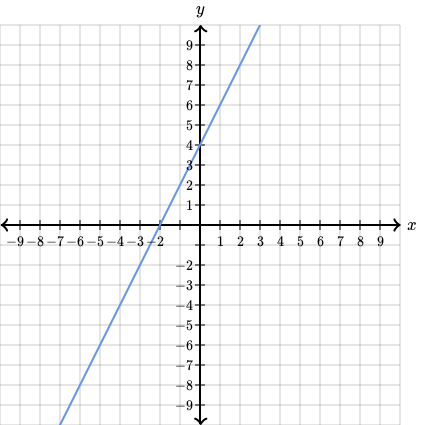
\includegraphics[scale=\shrinkfactor]{figures/c55256c02b190a7aba6f2a02fb7d6bf49a8652da.png}

**What is the equation that describes $y$ as a function of $x$?**

\paragraph{Ans}The equation \DIFdelbegin \DIFdel{which }\DIFdelend \DIFaddbegin \DIFadd{that }\DIFaddend describes $y$ as a function of $x$ is 
[[? expression 1]] y = 2x+4

\paragraph{Hint 1}We are shown the graph of a function, and we want to find the \DIFdelbegin \DIFdel{function which }\DIFdelend \DIFaddbegin \DIFadd{equation that }\DIFaddend corresponds to this graph. In other words, we are looking for the equation \DIFdelbegin \DIFdel{which }\DIFdelend \DIFaddbegin \DIFadd{that }\DIFaddend describes $\blue{y}$ as a function of $\red{x}$.

Observe that the slope of the graph is equal to $\purple{2}$ and its $y$-intercept is $\green{4}$.
Let's use this information to figure out the equation \DIFdelbegin \DIFdel{which }\DIFdelend \DIFaddbegin \DIFadd{that }\DIFaddend corresponds to this graph.

\paragraph{Hint 2}The graph of this line passes through the point $(0,\green{4})$. We say the $y$-intercept of the graph is equal to $\green{4}$. This is where the graph crosses the $y$-axis. The $y$-intercept of the graph tells us the initial value of the function. When $\red{x}=0$, $\blue{y}=\green{4}$.

\paragraph{Hint 3}Now, let's see how to interpret the slope of the function. The slope of the graph tells us how $\blue{y}$ changes when $\red{x}$ changes. Observe that when $\red{x}$ changes from $\red{0}$ to $\red{1}$,
$\blue{y}$ changes from $\blue{4}$ to $\blue{6}$.
Also when $\red{x}$ changes from $\red{1}$ to $\red{2}$, $\blue{y}$ changes from $\blue{6}$ to $\blue{8}$. The change in $\blue{y}$ is equal to \DIFdelbegin \DIFdel{two }\DIFdelend \DIFaddbegin \DIFadd{$\purple{2}$ }\DIFaddend times the change in $\red{x}$.

Now that we know the initial value of the function and its rate of change we can write the equation \DIFdelbegin \DIFdel{which }\DIFdelend \DIFaddbegin \DIFadd{that }\DIFaddend describes $\blue{y}$ as a function of $\red{x}$

$\quad \blue{y} = \purple{2}\red{x} + \green{4}$.


\paragraph{Hint 4}Let's check that this equation correctly describes the function by verifying some $(\red{x},\blue{y})$ pairs. 

When $\red{x}=\red{0}$, the equation for $\blue{y}$ gives $\blue{y}=\purple{2}(\red{0}) + \green{4} = \blue{4}$. This corresponds to the point $(\red{0},\blue{4})$ which is part of the graph of the function.

Also, when $\red{x}=\red{1}$, $\blue{y}=\purple{2}(\red{1}) + \green{4}=\blue{6}$.  The point $(\red{1},\blue{6})$ is also part of the graph of the function.

Finally, when $\red{x}=\red{2}$, the equation correctly predicts $\blue{y}=\purple{2}(\red{2}) + \green{4}=\blue{8}$. 

\paragraph{Hint 5}The equation \DIFdelbegin \DIFdel{which }\DIFdelend \DIFaddbegin \DIFadd{that }\DIFaddend describes $y$ as a function of $x$ is $y = 2x + 4$.



\medskip
\noindent
\textbf{Tags:} {\footnotesize CC.8.F.B.4, SB.8.1.F.1.CR, Constructing linear functions.3}\\
\textbf{Version:} \DIFdelbegin \DIFdel{c9cd8189.. 2013-08-13
}\DIFdelend \DIFaddbegin \DIFadd{773efde9.. 2013-08-19
}\DIFaddend \smallskip\hrule





\section{\href{https://www.khanacademy.org/devadmin/content/items/x4d8feb39}{x4d8feb39}}

\noindent
Sean works in sales. His monthly salary $S$ depends on his sales performance. The graph below shows his salary as a function of the number of sales $n$  he makes during the month.

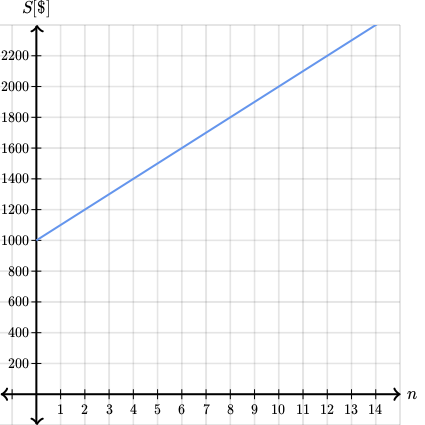
\includegraphics[scale=\shrinkfactor]{figures/88f55c935fe40d38b0894522ee4c9ee3e18982d9.png}

**Find the equation \DIFdelbegin \DIFdel{which }\DIFdelend \DIFaddbegin \DIFadd{that }\DIFaddend describes Sean's monthly salary $S$ as a function of the number of sales $n$.**

\paragraph{Ans}The equation \DIFdelbegin \DIFdel{which }\DIFdelend \DIFaddbegin \DIFadd{that }\DIFaddend describes Sean's salary $S$ as a function of the number of sales $n$ is  
[[? expression 1]] S= 1000+100*n

\paragraph{Hint 1}We're shown the graph of the function \DIFdelbegin \DIFdel{which }\DIFdelend \DIFaddbegin \DIFadd{that }\DIFaddend describes how Sean's monthly salary $\blue{S}$ depends on the number of sales $\red{n}$. Let's use the information from the graph to figure out the equation \DIFdelbegin \DIFdel{which }\DIFdelend \DIFaddbegin \DIFadd{that }\DIFaddend represents $\blue{S}$ as a function of $\red{n}$.

\paragraph{Hint 2}Looking at the graph we see that the initial value of the function $\blue{S}$ is $\$\green{1000}$. Even if Sean makes $\red{n}=0$ sales, he will still receive a monthly salary of $\$\green{1000}$. 

\paragraph{Hint 3}Next, let's look at the slope of the graph. If Sean makes $\red{x}=\red{2}$ sales, his salary will be $\blue{S}=\$\blue{1200}$. Thus, a change of $\red{2}$ in the number of sales $\red{n}$ produces a change of $\$\blue{200}$ in the salary $\blue{S}$. The rate of change of the salary function is:

$\quad 
\purple{m} = \dfrac{ \textrm{change in } \blue{S} }{ \textrm{change in } \red{n} } = 
\dfrac{ \blue{1200} - \blue{1000} }{ \red{2} - \red{0} } 
= \dfrac{200}{2} = \purple{100}$.

Sean's salary increases by $\$\purple{100}$ for each sale he makes. 

\paragraph{Hint 4}Combining all the information we have about Sean's monthly salary, we can now write his salary $\blue{S}$ as a function of the number of sales $\red{n}$ as follows:

\begin{align*}
\quad \blue{S} 
&=  \green{1000} + \purple{100}\red{n}.
\end{align*}

\paragraph{Hint 5}Note that the salary $\blue{S}$ is described by a *linear equation* $\blue{S}=\green{b}+\purple{m}\cdot\red{n}$, where $\green{b}=\green{1000}$ represents the initial value of the function and $\purple{m}=\purple{100}$ represents the rate of change of the function.

The graph of the function $\blue{S}=\green{1000} + \purple{100}\red{n}$ is a *line* \DIFdelbegin \DIFdel{which }\DIFdelend \DIFaddbegin \DIFadd{that }\DIFaddend passes through the point $(\red{0},\blue{1000})$ and has slope equal to $\purple{100}$. We can understand the function \DIFdelbegin \DIFdel{which }\DIFdelend \DIFaddbegin \DIFadd{that }\DIFaddend describes Sean's salary either through its equation or through its graph.

\paragraph{Hint 6}The equation \DIFdelbegin \DIFdel{which }\DIFdelend \DIFaddbegin \DIFadd{that }\DIFaddend describes Sean's salary $S$ as a function of the number of sales $n$ is  $S = 1000+100n$.



\medskip
\noindent
\textbf{Tags:} {\footnotesize CC.8.F.B.4, SB.8.1.F.1.CR, Constructing linear functions.3}\\
\textbf{Version:} \DIFdelbegin \DIFdel{68b6bf09.. 2013-08-13
}\DIFdelend \DIFaddbegin \DIFadd{dafe08ad.. 2013-08-19
}\DIFaddend \smallskip\hrule





\section{\href{https://www.khanacademy.org/devadmin/content/items/x4eabf393}{x4eabf393}}

\noindent
Jimmy will be selling hot dogs at the football game. He bought hot dogs, buns and condiments for $\$8$ before the game and now he wants to calculate the profit he will make. The graph below shows how Jimmy's profit $P\:$ depends on the number of hot dogs he sells at the game.

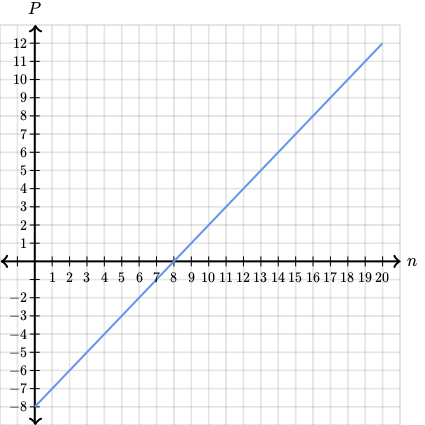
\includegraphics[scale=\shrinkfactor]{figures/2d882eb9739295abe5dc10510ecf8f2564fd633e.png}

**Write the equation \DIFdelbegin \DIFdel{which }\DIFdelend \DIFaddbegin \DIFadd{that }\DIFaddend describes Jimmy's profit $P\:$ as a function of the number $n$ of hot dogs sold.**

\paragraph{Ans}The equation \DIFdelbegin \DIFdel{which }\DIFdelend \DIFaddbegin \DIFadd{that }\DIFaddend describes Jimmy's profit $P$ as a function of the number of hot dogs sold $n$ is   
[[? expression 1]] P = 1*n-8

\paragraph{Hint 1}The graph shows how the profit $\blue{P}\:$ varies as a function of the number of hot dogs sold $\red{n}$. Let's see how to use the graph of the function to find the equation of the function.

\paragraph{Hint 2}Looking at the graph, we see the initial value of the profit function is $\green{-8}$ dollars. If Jimmy doesn't sell any hot dogs ($\red{n}=0$), his profit will be $\green{-8}$ dollars. A negative profit is a *loss*. 
Indeed, if Jimmy doesn't sell any hot dogs he will lose the money he invested to buy the ingredients.

\paragraph{Hint 3}Next, observe the slope of the graph is equal to $\purple{1}$. For each hot dog sold, the profit increases by $\$\purple{1}$. This means Jimmy is selling the hot dogs for $\$\purple{1}$ each.

\paragraph{Hint 4}Combining these facts about Jimmy's hot dog operation, we can now write his profit $\blue{P}$ as a function of the number of sales $\red{n}$ as follows:

\begin{align*}
\quad \blue{P} 
&=   \DIFdelbegin %DIFDELCMD < \green{-8} %%%
\DIFdel{+ }\DIFdelend \purple{1}\red{n} \DIFaddbegin \green{-8}\DIFaddend .
\end{align*}


\paragraph{Hint 5}Note that the profit $\blue{P}\:$ is described by a *linear equation* $\blue{P}=\purple{m}\cdot\red{n}  + \green{b}$, where $\green{b}=\green{-8}$ represents Jimmy's initial investment and $\purple{m}=\purple{1}$ represents sale price of each hot dog.

The graph of the function \DIFdelbegin \DIFdel{$\blue{P}=\green{-8} + \purple{1}\red{n}$ }\DIFdelend \DIFaddbegin \DIFadd{$\blue{P}=\purple{1}\red{n} \green{-8}$ }\DIFaddend is a *line* \DIFdelbegin \DIFdel{which }\DIFdelend \DIFaddbegin \DIFadd{that }\DIFaddend passes through the point $(\red{0},\blue{-8})$ and has slope equal to $\purple{1}$. We can understand the function \DIFdelbegin \DIFdel{which }\DIFdelend \DIFaddbegin \DIFadd{that }\DIFaddend describes Jimmy's profit either through its equation or through its graph.

\paragraph{Hint 6}The equation \DIFdelbegin \DIFdel{which }\DIFdelend \DIFaddbegin \DIFadd{that }\DIFaddend describes Jimmy's profit $P$ as a function of the number of hot dogs sold $n$ is  \DIFdelbegin \DIFdel{$P = -8+1\cdot n$}\DIFdelend \DIFaddbegin \DIFadd{$P = 1\cdot n - 8$}\DIFaddend .



\medskip
\noindent
\textbf{Tags:} {\footnotesize CC.8.F.B.4, SB.8.1.F.1.CR, Constructing linear functions.3}\\
\textbf{Version:} \DIFdelbegin \DIFdel{0b5a609b.. 2013-08-07
}\DIFdelend \DIFaddbegin \DIFadd{8471638c.. 2013-08-19
}\DIFaddend \smallskip\hrule





\section{\href{https://www.khanacademy.org/devadmin/content/items/x5ced1189}{x5ced1189}}

\noindent
Kristina is organizing a music concert. She plans to invest $\$2000$ to rent the venue and to pay the musicians and then sell the tickets for $\$20$ each. The graph below shows the profit $P\:$ she will make from the concert as a function of the number of tickets sold $n$.

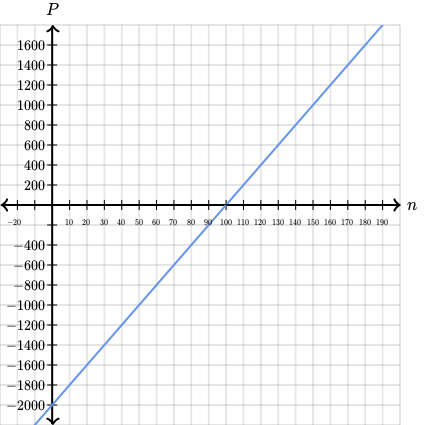
\includegraphics[scale=\shrinkfactor]{figures/12887f1c5619e9b66cfbad5ad051ba5d1bd078d8.png}

**What is the equation \DIFdelbegin \DIFdel{which }\DIFdelend \DIFaddbegin \DIFadd{that }\DIFaddend describes $P$ as a function of $n$?**

\paragraph{Ans}The equation \DIFdelbegin \DIFdel{which }\DIFdelend \DIFaddbegin \DIFadd{that }\DIFaddend describes Kristina's profit $P$ as a function of the number of tickets $n$ is 
[[? expression 1]] P = 20*n  - 2000

\paragraph{Hint 1}The graph shows how the profit $\blue{P}\:$ varies as a function of the number of tickets sold $\red{n}$. Let's use the information from the graph to figure out the equation \DIFdelbegin \DIFdel{which }\DIFdelend \DIFaddbegin \DIFadd{that }\DIFaddend describes $\blue{P}\:$ as a function of $\red{n}$.

\paragraph{Hint 2}The slope of the graph is equal to $\purple{20}$
since Kristina is selling the tickets for $\$\purple{20}$ each. 

We can confirm this is the case by looking at the graph. Each time the number of tickets sold increases by $\red{10}$, the graph of Kristina's profits increases by $\$\blue{200}$.

\paragraph{Hint 3}If Kristina sells $\red{n}=0$ tickets, then the profit will be $\blue{P}=\green{-2000}$. In other words, Kristina will not have a profit but a *loss*. Her loss is equal to the $\$\green{2000}$ she invested to organize the concert.

\paragraph{Hint 4}**The equation that describes Kristina's profit $\blue{P}\:$ as a function of the number of tickets sold $\red{n}$ is **

\begin{align*}
\qquad \blue{P} 
  &=\purple{m}\red{n}+\green{b} \\
  &=\purple{20}\cdot \red{n} \green{-2000}
\end{align*}  

\DIFdelbegin \paragraph{\DIFdel{Hint 5}}%DIFAUXCMD
\addtocounter{paragraph}{-1}%DIFAUXCMD
\DIFdelend The rate of change $\purple{m}=\purple{20}$ corresponds to the price $\$\purple{20}$ per ticket, and the initial value $\green{b=-2000}$ corresponds to Kristina's initial investment of $\$\green{2000}$\DIFdelbegin \DIFdel{**.
**
}\DIFdelend \DIFaddbegin \DIFadd{.
}\DIFaddend 



\medskip
\noindent
\textbf{Tags:} {\footnotesize CC.8.F.B.4, SB.8.1.F.1.CR, Constructing linear functions.3}\\
\textbf{Version:} \DIFdelbegin \DIFdel{2efa29f4.. 2013-08-12
}\DIFdelend \DIFaddbegin \DIFadd{3800680d.. 2013-08-19
}\DIFaddend \smallskip\hrule





\section{\href{https://www.khanacademy.org/devadmin/content/items/x64530386}{x64530386}}

\noindent
Jeff works as a waiter at a fancy restaurant. Assume $n$ represents the number of clients Jeff will serve in a day and $E$ represents his daily earnings.
The graph that represents Jeff's daily earnings as a function of the number of clients he serves is shown below.

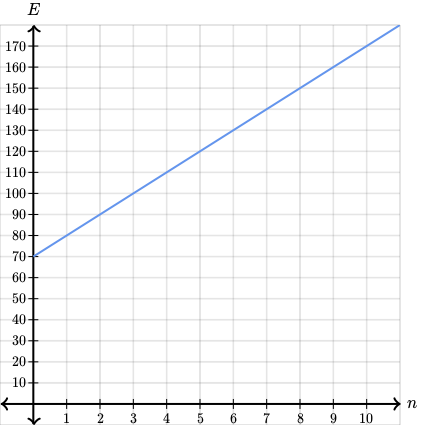
\includegraphics[scale=\shrinkfactor]{figures/d96601972ab5c577e1fe0bbae8a2e74677fadf55.png}

**What is the equation \DIFdelbegin \DIFdel{which }\DIFdelend \DIFaddbegin \DIFadd{that }\DIFaddend describes $E$ as a function of $n$?**

\paragraph{Ans}The equation \DIFdelbegin \DIFdel{which }\DIFdelend \DIFaddbegin \DIFadd{that }\DIFaddend describes Jeff's earnings $E$ as a function of the number of clients $n$ is 
 [[? expression 1]] E = 70 + 10*n

\paragraph{Hint 1}We\DIFaddbegin \DIFadd{'}\DIFaddend re looking for the equation \DIFdelbegin \DIFdel{which }\DIFdelend \DIFaddbegin \DIFadd{that }\DIFaddend corresponds to the graph. We want to find the function \DIFdelbegin \DIFdel{which }\DIFdelend \DIFaddbegin \DIFadd{that }\DIFaddend describes how Jeff's daily earnings $\blue{E}$ depends on the number of clients he serves $\red{n}$.

\paragraph{Hint 2}By looking at the graph, we see that Jeff's earnings $\blue{E}$ increase by $\$\purple{10}$ for each client he serves.  Also, note that Jeff receives a base daily salary of $\$\green{70}$.

So overall, Jeff receives a base amount of $\$\green{70}$ each day, plus approximately $\$\purple{10}$  tip for each client he serves. 

\paragraph{Hint 3}Jeff's daily earnings $\blue{E}$ as a function of the number of clients he serves $\red{n}$ is described by the following linear equation:

\begin{align*}
\quad \blue{E} 
 &= \green{b}   + \purple{m}\cdot\red{n}  \\[1mm]
 &= \green{70}   +  \purple{10}\cdot\red{n}.
\end{align*}

The initial value is $\green{b=70}$. This is the base amount Jeff earns even when he serves $\red{n}=0$ clients.

The rate of change is $\purple{m}=\purple{10}$ because this is how much tip he makes per client. If $\red{n}$ increases by one, his salary $\blue{E}$ will increase by $\$\purple{10}$. 


\paragraph{Hint 4}The equation \DIFdelbegin \DIFdel{which }\DIFdelend \DIFaddbegin \DIFadd{that }\DIFaddend describes Jeff's earnings $E$ (in dollars) as a function of the number of clients $n$ is $E = 70 + 10n$.



\medskip
\noindent
\textbf{Tags:} {\footnotesize CC.8.F.B.4, SB.8.1.F.1.CR, Constructing linear functions.3}\\
\textbf{Version:} \DIFdelbegin \DIFdel{d3a875d3.. 2013-08-13
}\DIFdelend \DIFaddbegin \DIFadd{9d66be47.. 2013-08-19
}\DIFaddend \smallskip\hrule





\section{\href{https://www.khanacademy.org/devadmin/content/items/x66af7067}{x66af7067}}

\noindent
Covi is driving from Montreal to New York City. The graph below shows his position $x$, measured in kilometers from the Canada-US border, as a function of time $t$, measured in hours.

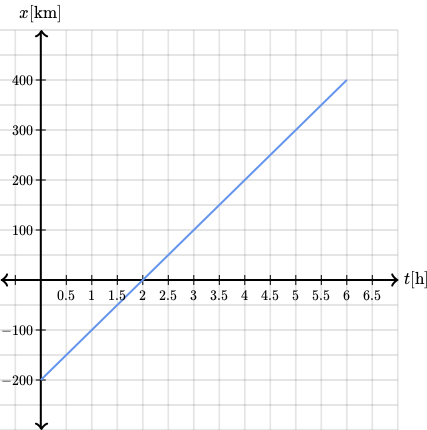
\includegraphics[scale=\shrinkfactor]{figures/e8fa2c2d06cffc6ef871bbc124814ca2d111357d.png}

**What is the equation that describes $x$ as a function of $t$?**

\paragraph{Ans}The equation \DIFdelbegin \DIFdel{which }\DIFdelend \DIFaddbegin \DIFadd{that }\DIFaddend describes $x$ as a function of $t$ is 
[[? expression 1]] x = -200+100*t

\paragraph{Hint 1}We are shown the graph of Covi's position $\blue{x}$ as a function of time $\red{t}$. We want to find the equation that corresponds to this graph.

\paragraph{Hint 2}In this graph $\blue{x}$ describes the position relative to the Canada-US border. Negative values of $\blue{x}$ correspond to locations in Canada, while positive values of $\blue{x}$ correspond to locations in the US.

Looking at the graph we see that Covi's initial position is $\green{-200}\text{ km}$. This is Covi's position when he starts from Montreal.

\paragraph{Hint 3}Next, let's find the slope of the graph. During the first $\red{1}$ hour, Covi's position changes by $\blue{100}\text{ km}$. A change of $\red{1}$ hour in the time $\red{t}$ produces a change of $\blue{100}\text{ km}$ in the position $\blue{x}$. The *rate of change* of the position is:

$\quad 
\purple{m} = \dfrac{ \textrm{change in } \blue{x} }{ \textrm{change in } \red{t} } = 
\dfrac{ (\blue{-100}) - (\blue{-200}) \text{ [km]}}{ \red{1} - \red{0} \text{ [h]}} 
= \dfrac{100\text{ km}}{1\text{ h}} = \purple{100}\text{ km/h}$.

Covi's position increases at a rate of $\purple{100}\text{ km/h}$. Note that the *rate of change* of the position function corresponds to a *velocity*. This makes sense if you think about it: if Covi is traveling at $\purple{100}\text{ km/h}$, then his position will change by $100 \text{ km}$ each hour.

\paragraph{Hint 4}We can now combine the information about the initial value and the rate of change to obtain the equation \DIFdelbegin \DIFdel{which }\DIFdelend \DIFaddbegin \DIFadd{that }\DIFaddend describes Covi's position as a function of time:

$\quad \blue{x} = \purple{100}\red{t}  \green{-200}$.

Note that Covi's position function is described by a linear equation $\blue{x} = \purple{m}\red{t} + \green{b}$, where $\purple{m}=\purple{100}\text{ km/h}$ describes the rate of change of Covi's position, and $\green{b}=\green{-200}\text{ km}$ describes Covi's initial position. 

\paragraph{Hint 5}The equation \DIFdelbegin \DIFdel{which }\DIFdelend \DIFaddbegin \DIFadd{that }\DIFaddend describes $x$ as a function of $t$ is  $x = 100t - 200$.



\medskip
\noindent
\textbf{Tags:} {\footnotesize CC.8.F.B.4, SB.8.1.F.1.CR, Constructing linear functions.3}\\
\textbf{Version:} \DIFdelbegin \DIFdel{5eb1757f.. 2013-08-13
}\DIFdelend \DIFaddbegin \DIFadd{78a03650.. 2013-08-19
}\DIFaddend \smallskip\hrule





\section{\href{https://www.khanacademy.org/devadmin/content/items/xba68007f}{xba68007f}}

\noindent
You are downloading a file from the Internet.
Assume $t$ represents the time in minutes, and $f$ represents the file size downloaded in $\text{MB}$. The following graph represents the file size as a function of time.

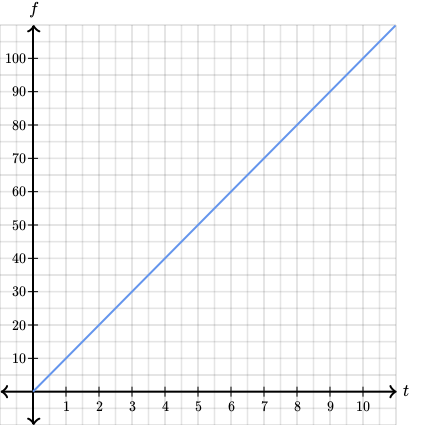
\includegraphics[scale=\shrinkfactor]{figures/1f1edf7a5ef2afc94d7bc7a5c8167b4150541603.png}

**What is the equation \DIFdelbegin \DIFdel{which }\DIFdelend \DIFaddbegin \DIFadd{that }\DIFaddend describes the file size $f$ as a function of $t$?**

\paragraph{Ans}The equation \DIFdelbegin \DIFdel{which }\DIFdelend \DIFaddbegin \DIFadd{that }\DIFaddend describes the growing file size $f$ (in $\text{MB}$) as a function of the time $t$ (in minutes) is 
[[? expression 1]] f = 10*t

\paragraph{Hint 1}We�re looking for the equation \DIFdelbegin \DIFdel{which }\DIFdelend \DIFaddbegin \DIFadd{that }\DIFaddend corresponds to the graph of the function.  We want to find the equation \DIFdelbegin \DIFdel{which }\DIFdelend \DIFaddbegin \DIFadd{that }\DIFaddend describes how the file size $\blue{f}$ grows with time $\red{t}$. 

\paragraph{Hint 2}The amount of downloaded data $\blue{f}$ is *proportional* to the time $\red{t}$. The constant of proportionality is $\purple{m}=\purple{10}\text{ MB/min}$, since this is the download rate. Indeed, a download speed of $\purple{10}\text{ MB/min}$ means the file size increases by $\purple{10}\text{ MB}$ each minute as we see in the graph.

\paragraph{Hint 3}If we want to describe $\blue{f}$ as a function of $\red{t}$, we can use the following equation:

\begin{align*}
\quad \blue{f} 
 &= \purple{m}\cdot\red{t} \\[1mm]
 &= \purple{10}\red{t}.
\end{align*}

\paragraph{Hint 4}Note that the *proportional relationship* of the form  $\blue{y} =\purple{m}\red{x}$ is a special case of the more general linear equation $\blue{y} =\purple{m}\red{x}+\green{b}$, with zero initial value $\green{b}=0$.

\paragraph{Hint 5}The equation \DIFdelbegin \DIFdel{which }\DIFdelend \DIFaddbegin \DIFadd{that }\DIFaddend describes the growing file size $f$ (in $\text{MB}$) as a function of the time $t$ (in minutes) is $f = 10t$.



\medskip
\noindent
\textbf{Tags:} {\footnotesize CC.8.F.B.4, SB.8.1.F.1.CR, Constructing linear functions.3}\\
\textbf{Version:} \DIFdelbegin \DIFdel{213b5bcc.. 2013-08-12
}\DIFdelend \DIFaddbegin \DIFadd{bb9fc9ad.. 2013-08-19
}\DIFaddend \smallskip\hrule



%%  Create a directory called 'figures' in latex dir and run the following command 
%  wget \
%    https://ka-perseus-graphie.s3.amazonaws.com/c55256c02b190a7aba6f2a02fb7d6bf49a8652da.png \
%    https://ka-perseus-graphie.s3.amazonaws.com/88f55c935fe40d38b0894522ee4c9ee3e18982d9.png \
%    https://ka-perseus-graphie.s3.amazonaws.com/2d882eb9739295abe5dc10510ecf8f2564fd633e.png \
%    https://ka-perseus-graphie.s3.amazonaws.com/12887f1c5619e9b66cfbad5ad051ba5d1bd078d8.png \
%    https://ka-perseus-graphie.s3.amazonaws.com/d96601972ab5c577e1fe0bbae8a2e74677fadf55.png \
%    https://ka-perseus-graphie.s3.amazonaws.com/e8fa2c2d06cffc6ef871bbc124814ca2d111357d.png \
%    https://ka-perseus-graphie.s3.amazonaws.com/1f1edf7a5ef2afc94d7bc7a5c8167b4150541603.png \


\end{document}
